\documentclass{egpubl}
\usepackage{eurovis2021}

% --- for  Annual CONFERENCE
% \ConferenceSubmission   % uncomment for Conference submission
% \ConferencePaper        % uncomment for (final) Conference Paper
% \STAR                   % uncomment for STAR contribution
% \Tutorial               % uncomment for Tutorial contribution
% \ShortPresentation      % uncomment for (final) Short Conference Presentation
% \Areas                  % uncomment for Areas contribution
% \MedicalPrize           % uncomment for Medical Prize contribution
% \Education              % uncomment for Education contribution
% \Poster                 % uncomment for Poster contribution
% \DC                     % uncomment for Doctoral Consortium
%
% --- for  CGF Journal
% \JournalSubmission    % uncomment for submission to Computer Graphics Forum
% \JournalPaper         % uncomment for final version of Journal Paper
%
% --- for  CGF Journal: special issue
% \SpecialIssueSubmission    % uncomment for submission to , special issue
\SpecialIssuePaper         % uncomment for final version of Computer Graphics Forum, special issue
%                          % EuroVis, SGP, Rendering, PG
% --- for  EG Workshop Proceedings
% \WsSubmission      % uncomment for submission to EG Workshop
% \WsPaper           % uncomment for final version of EG Workshop contribution
% \WsSubmissionJoint % for joint events, for example ICAT-EGVE
% \WsPaperJoint      % for joint events, for example ICAT-EGVE
% \Expressive        % for SBIM, CAe, NPAR
% \DigitalHeritagePaper
% \PaperL2P          % for events EG only asks for License to Publish

% --- for EuroVis 
% for full papers use \SpecialIssuePaper
% \STAREurovis   % for EuroVis additional material 
% \EuroVisPoster % for EuroVis additional material 
% \EuroVisShort  % for EuroVis additional material

% !! *please* don't change anything above
% !! unless you REALLY know what you are doing
% ------------------------------------------------------------------------

\usepackage[T1]{fontenc}
\usepackage{dfadobe}


% \usepackage{cite}  % comment out for biblatex with backend=biber
% ---------------------------
\biberVersion
\BibtexOrBiblatex
\usepackage[backend=biber,bibstyle=EG,citestyle=alphabetic,backref=true,url=false]{biblatex}
%\addbibresource{egbibsample.bib}

\renewbibmacro*{doi+eprint+url}{%
    \printfield{doi}%
    \newunit\newblock%
    \iftoggle{bbx:eprint}{%
        \usebibmacro{eprint}%
    }{}%
    \newunit\newblock%
    \iffieldundef{doi}{%
        \usebibmacro{url+urldate}}%
        {}%
    }

\addbibresource{GeoVis.bib}

\newcommand{\citetitlea}[1]{\citefield{#1}{title}}

% ---------------------------  
\electronicVersion
\PrintedOrElectronic
% for including postscript figures
% mind: package option 'draft' will replace PS figure by a filename within a frame
\ifpdf \usepackage[pdftex]{graphicx} \pdfcompresslevel=9
\else \usepackage[dvips]{graphicx} \fi

\usepackage{egweblnk}
% end of prologue

\usepackage{float,hhline,hyperref,array,tabulary,tabularx,etoolbox,multirow}

\newcommand{\algorithmautorefname}{Algorithm}

\usepackage{dblfloatfix}

\usepackage[table, dvipsnames]{xcolor}

\usepackage{multicol}

% auto labeling of sections
\let\origsection=\section
\renewcommand\section[1]{\origsection{#1}\label{sec:{#1}}}

\let\origsubsection=\subsection
\renewcommand\subsection[1]{\origsubsection{#1}\label{subsec:{#1}}}

\let\origsubsubsection=\subsubsection
\renewcommand\subsubsection[1]{\origsubsubsection{#1}\label{subsubsec:{#1}}}

% cite with author names
\newcommand{\citea}[1]{\citeauthor{#1}~\cite{#1}}

% software name
\newcommand{\software}{GHRVis}

% Bob's dream paragraph style
\newcommand{\bobgraph}[1]{ \noindent\textbf{#1} \phantomsection \label{bobgraph:{#1}}}

\definecolor{Mycolor1}{HTML}{4C5866} %#4C5866
\definecolor{Mycolor2}{HTML}{A6B6D2} %#A6B6D2
\definecolor{Mycolor3}{HTML}{67daff} %#67daff
\definecolor{Mycolor4}{HTML}{F7F7FE} %#F7F7FE
\definecolor{Mycolor5}{HTML}{666ad1} %#666ad1
\definecolor{Mycolor6}{HTML}{ffbb93} %#ffbb93
\newcommand{\mycolorbox}[2]{\begingroup\setlength{\fboxsep}{2pt}\colorbox{#1}{#2}\endgroup}

% customized table headers
\newcommand{\theaderR}[1]{\multicolumn{1}{c|}{\cellcolor{Mycolor3} \textbf{\rotatebox{90}{#1 \phantom{-} }}}}
\newcommand{\theaderP}[1]{\cellcolor{Mycolor3} \textbf{#1}}

\newcommand{\note}[1]{\textcolor{blue}{#1}}


% thumbnail image
\usepackage{wrapfig}
\newcommand{\thumbnail}[2]{
      \setlength{\intextsep}{3pt}
      \setlength{\columnsep}{3pt}
      \begin{wrapfigure}{r}{0.2\columnwidth}
        \begin{center}
          \includegraphics[width=0.2\columnwidth]{figure/related/"#1".png}
        \end{center}
      \end{wrapfigure}
      #2
}


\usepackage{algpseudocode}
\usepackage{algorithm}
% switch for algorithmic
% New definitions
\algnewcommand\algorithmicswitch{\textbf{switch}}
\algnewcommand\algorithmiccase{\textbf{case}}
\algnewcommand\algorithmicdefault{\textbf{default}}

\algdef{SE}[SWITCH]{Switch}{EndSwitch}[1]{\algorithmicswitch\ #1\textbf{:}}{\algorithmicend\ \algorithmicswitch}%
\algtext*{EndSwitch}%

\algdef{SE}[CASE]{Case}{EndCase}[1]{\algorithmiccase\ #1\textbf{:}}{\algorithmicend\ \algorithmiccase}%
\algtext*{EndCase}%

\algdef{SE}[DEFUALT]{Default}{EndDefault}{\algorithmicdefault\textbf{:}}{\algorithmicend\ \algorithmicdefault}%
\algtext*{EndDefault}%

\algnewcommand\algorithmicforeach{\textbf{for each}}
\algdef{S}[FOR]{ForEach}[1]{\algorithmicforeach\ #1\ \algorithmicdo}

% code listing

\usepackage{listings}
\lstdefinestyle{customc}{
  belowcaptionskip=1\baselineskip,
  breaklines=true,
  xleftmargin=\parindent,
  language=C,
  showstringspaces=false,
  basicstyle=\footnotesize\ttfamily,
  keywordstyle=\bfseries\color{green!40!black},
  commentstyle=\itshape\color{purple!40!black},
  identifierstyle=\color{blue},
  stringstyle=\color{orange},
}

\lstdefinestyle{customasm}{
  belowcaptionskip=1\baselineskip,
  xleftmargin=\parindent,
  language=[x86masm]Assembler,
  basicstyle=\footnotesize\ttfamily,
  commentstyle=\itshape\color{purple!40!black},
}

\lstset{escapechar=@,style=customc}
\usepackage{amsmath,bm}
\usepackage{amssymb}

% bold \mathcal{}
\DeclareMathAlphabet{\mathbcal}{OMS}{cmsy}{b}{n}

% wrapper for math symbols
\newcommand{\Vector}[1]{\protect\overrightarrow{#1}}
\newcommand{\Line}[1]{\protect\overline{#1}}
\newcommand{\dx}{\Delta x}
\newcommand{\dy}{\Delta y}
\newcommand{\Width}[1]{\lvert #1 \rvert}

% UpdateNodePosition
\newcommand{\nodeList}{\bm{L}}

\newcommand{\nodeStalemate}{\node.stalemate}

\newcommand{\nodeFNORLine}{\Line{\node\nodeFNOR}}
\newcommand{\nodeSize}{s}
\newcommand{\nodeSizeMax}{s_{max}}
\newcommand{\stalemateMax}{w}
\newcommand{\nodeCross}{\node.cross}
\newcommand{\nodeListCross}{\nodeList.cross}

% move position

\newcommand{\node}{\bm{n}}
\newcommand{\nodePrevious}{\node_{p}}
\newcommand{\nodeFNOR}{\node_t}

\newcommand{\nodeVectorTC}{\Vector{\nodeFNOR\node}}
\newcommand{\nodeVectorCT}{\Vector{\node\nodeFNOR}}

% check river crossing

\newcommand{\riverEdge}{\bm{r}}
\newcommand{\riverEdgeList}{\bm{R}}
\newcommand{\riverEdgeLine}{\Line{\riverEdge}}
\newcommand{\nodeBoundingBox}{b_n}
\newcommand{\riverEdgeBoundingBox}{b_{\riverEdge}}
\newcommand{\boundingBoxInt}{b_{int.}}
\newcommand{\nodeEdge}{e_n}
\newcommand{\edgeBoxInt}{e_{int.}}

% derive corridor
\newcommand{\Corridor}{c}
\newcommand{\CorridorLength}{\Corridor_l}
\newcommand{\CorridorWidth}{\Corridor_w}
\newcommand{\PointP}{\node_c}
\newcommand{\Edge}{\Line{e}}
\newcommand{\EdgeStart}{\Edge.start}
\newcommand{\EdgeEnd}{\Edge.end}
\newcommand{\EdgeParallel}{\Line{e_p}}
\newcommand{\EdgeParallelA}{\Line{e_{p^1}}}
\newcommand{\EdgeParallelB}{\Line{e_{p^2}}}
\newcommand{\Distance}{d}
\newcommand{\nodeVectorNP}{\Vector{\node\PointP}}
\newcommand{\nodeVectorNV}{\Vector{\node\nodeFNOR}}
\newcommand{\nodeLineNV}{\Line{\node\nodeFNOR}}
\newcommand{\nodeLinePN}{\Line{\nodePrevious\node}}
\newcommand{\nodeVectorNtP}{\Vector{\nodeFNOR\PointP}}
\newcommand{\nodeLineNtNc}{\Line{\nodeFNOR\PointP}}
\newcommand{\nodeLineWidthNtP}{\Width{\nodeFNOR\PointP}}
\newcommand{\nodeInCorridor}{\node_{in}}
\newcommand{\nodeInCorridorT}{\node_{in_t}}


% derive corridor point
\newcommand{\Scale}{scale}

% figure fig:corridor

\newcommand{\nodeVectorNNn}{\Vector{\node\node_{t}}}
\newcommand{\nodeVectorNinNinn}{\Vector{\nodeInCorridor\nodeInCorridorT}}

\newcommand{\new}[1]{\textcolor{blue}{#1}}

\author[Q. Wang \& R. S. Laramee]
{\parbox{\textwidth}{\centering Q. Wang
  and R. S. Laramee
    }
    \\
\parbox{\textwidth}{\centering School of Computer Science, University of Nottingham, UK}
}

\title{Cartograms with Dynamic Features}

\begin{document}

\pagestyle{plain}

\maketitle

\begin{abstract}
Cartograms are hybrid representations of geographical and abstract data based on a value-by-area mapping technique. Based on the Dorling cartogram, the Demers cartogram uses squares instead of circles to represent regions, enabling the comparison of regions in a more intuitive way with a higher screen space utilization. One of the disadvantages of the Dorling cartogram and its variants is that regions may be displaced from their original positions, reducing the legibility, readability, and geographical accuracy. To address that, we propose a novel layout algorithm that integrates dynamic topological features such as rivers into Demers cartograms. We evaluate the proposed layout algorithm through a user study with an application to an Electronic Health Records (EHR) dataset. The results demonstrate that the proposed layout algorithm is able to preserve some of the original properties of the cartogram, while improving the legibility, readability, and geographical accuracy of the cartogram. 
\end{abstract}

\section{Introduction and Motivation}

Cartograms are representations of hybrid geographical and abstract data based on a value-by-area mapping technique combining statistical and geographical information \cite{dent2009Cartography}. Various styles of cartograms have been proposed and implemented, covering applications such as urban planning \cite{harris2018Mapping, arranz-lopez2021Enduser}, natural hazard forecasting \cite{pappenberger2019Cartograms, park2020Flood}, conservation and environmental planning \cite{galluzzi2018Mapping, rocchini2019Cartogramming}, political and social demographics \cite{breitzman2018Using, alieva2021How}, and public health decision making \cite{gao2020Visualising, sack2021Visualizing}.

Among the four types of cartograms categorized by \citea{nusrat2016State} (contiguous, non-contiguous, rectangular, and Dorling), a trade-off between types of accuracy is made (See \tableref{table:accuracy}). For this project we focus on non-contiguous cartograms like Demers cartograms, because they facilitate statistical comparison between regions and they can make good use of screen space. Building on Demers cartograms \cite{ian2002Cartogram}, we introduce and develop novel dynamic topological features, such as rivers, aiming to improve the readability and geographical accuracy without sacrificing statistical accuracy. We implement a new cartographic layout algorithm that includes these topological features into the layout of the nodes representing geographical regions. To minimize geographical errors and make efficient use of screen space, the algorithm also updates the position of rivers to accommodate the node layout. We then apply the algorithm to a real world case-study using an Electronic Health Records (EHR) dataset to evaluate of our algorithm. We also present a user study demonstrating its effectiveness.

Our contributions include:

\begin{itemize}
    \item A new variant of Demers cartograms that incorporates dynamic topological features to improve readability and recognizability,
    \item A novel layout algorithm that preserves node positions relative to dynamic topological features such as rivers,
    \item A user study evaluation of the technique with an application to EHRs.
\end{itemize}

One of the major challenges involved is how to develop a layout algorithm that handles different shapes. In other words, the layout algorithm is novel because it handles different types of nodes -- rectangular representing regions and polylines representing rivers. Another challenge we overcome in developing the algorithm is to resolve stalemate situations introduced by dynamic topological features while minimizing the geographical error.

\section{Related Work}
\begin{table*}[!tb]
	\centering
	\resizebox{\textwidth}{!}{
		\begin{tabulary}{\textwidth}{|*{3}{l|}r|c|}
			\hhline{~|*{3}{-}|~}
			\multicolumn{1}{c|}{\textbf{Literature}} &
			\textbf{Title} &
			\textbf{Geographic Region} &
			\textbf{Number of Nodes} &
			\multicolumn{1}{c}{\textbf{Year}} \\
			\hline
			
			% \citea{auber2007Geographical} & \citetitlea{auber2007Geographical} & US & 19 & 2007 \\
			% \hline
			\citea{warf2008Geography} & \citetitlea{warf2008Geography} & US & 3,142 & \citeyear{warf2008Geography} \\
			\hline
			\citea{sun2010Effectiveness} & \citetitlea{sun2010Effectiveness} & US, China & 34 - 49 & \citeyear{sun2010Effectiveness} \\
			\hline
			\citea{cruz2017Adapted} & \citetitlea{cruz2017Adapted} & Portugal & 2,882 & \citeyear{cruz2017Adapted} \\
			\hline
			\citea{tong2018cartograms} & \citetitlea{tong2018cartograms} & England & 209 & \citeyear{tong2018cartograms} \\
			\hline
			\citea{gao2020Visualising} & \citetitlea{gao2020Visualising} & China & 34 & \citeyear{gao2020Visualising} \\
			\hline
			\citea{nusrat2020Recognition} & \citetitlea{nusrat2020Recognition} & Portugal & 49 & \citeyear{nusrat2020Recognition} \\
			\hline
			



			% \multicolumn{1}{c|}{\textbf{Total unique papers: 51}} & 24&15&12& \multicolumn{1}{c}{}  \\
			% \hhline{~|*{3}{-}|~}

		\end{tabulary}
	}
	\caption{Discuss Demers cartogram}
	\label{table:challenge table}
\end{table*}

\section{Data Description}

Obtaining the heterogenous data can be challenging, especially when an Electronic Health Records (EHR) dataset is involved \cite{wang2021EHRa}. The data acquisition involves multiple steps. The first step is to obtain both geospatial boundaries and EHR data that match one another. The second step is to pre-process the EHR data to remove empty and erroneous values. The final step is to transform the data into a format that is suitable for visualization.

\subsection{Geospatial Data}

Geospatial boundaries, or shapefiles, were obtained from the following sources. After acquiring the shapefiles, we used QGIS \cite{qgisWelcome} to manually adjust projections and merge them into one shapefile. Finally, mapshaper \cite{blochMapshaper} is used to convert the merged shapefile into a TopoJSON \cite{TopoJSON} file to reduce the file size and improve the performance of our implementation.

{
\begin{figure}[tb!]
    \centering
    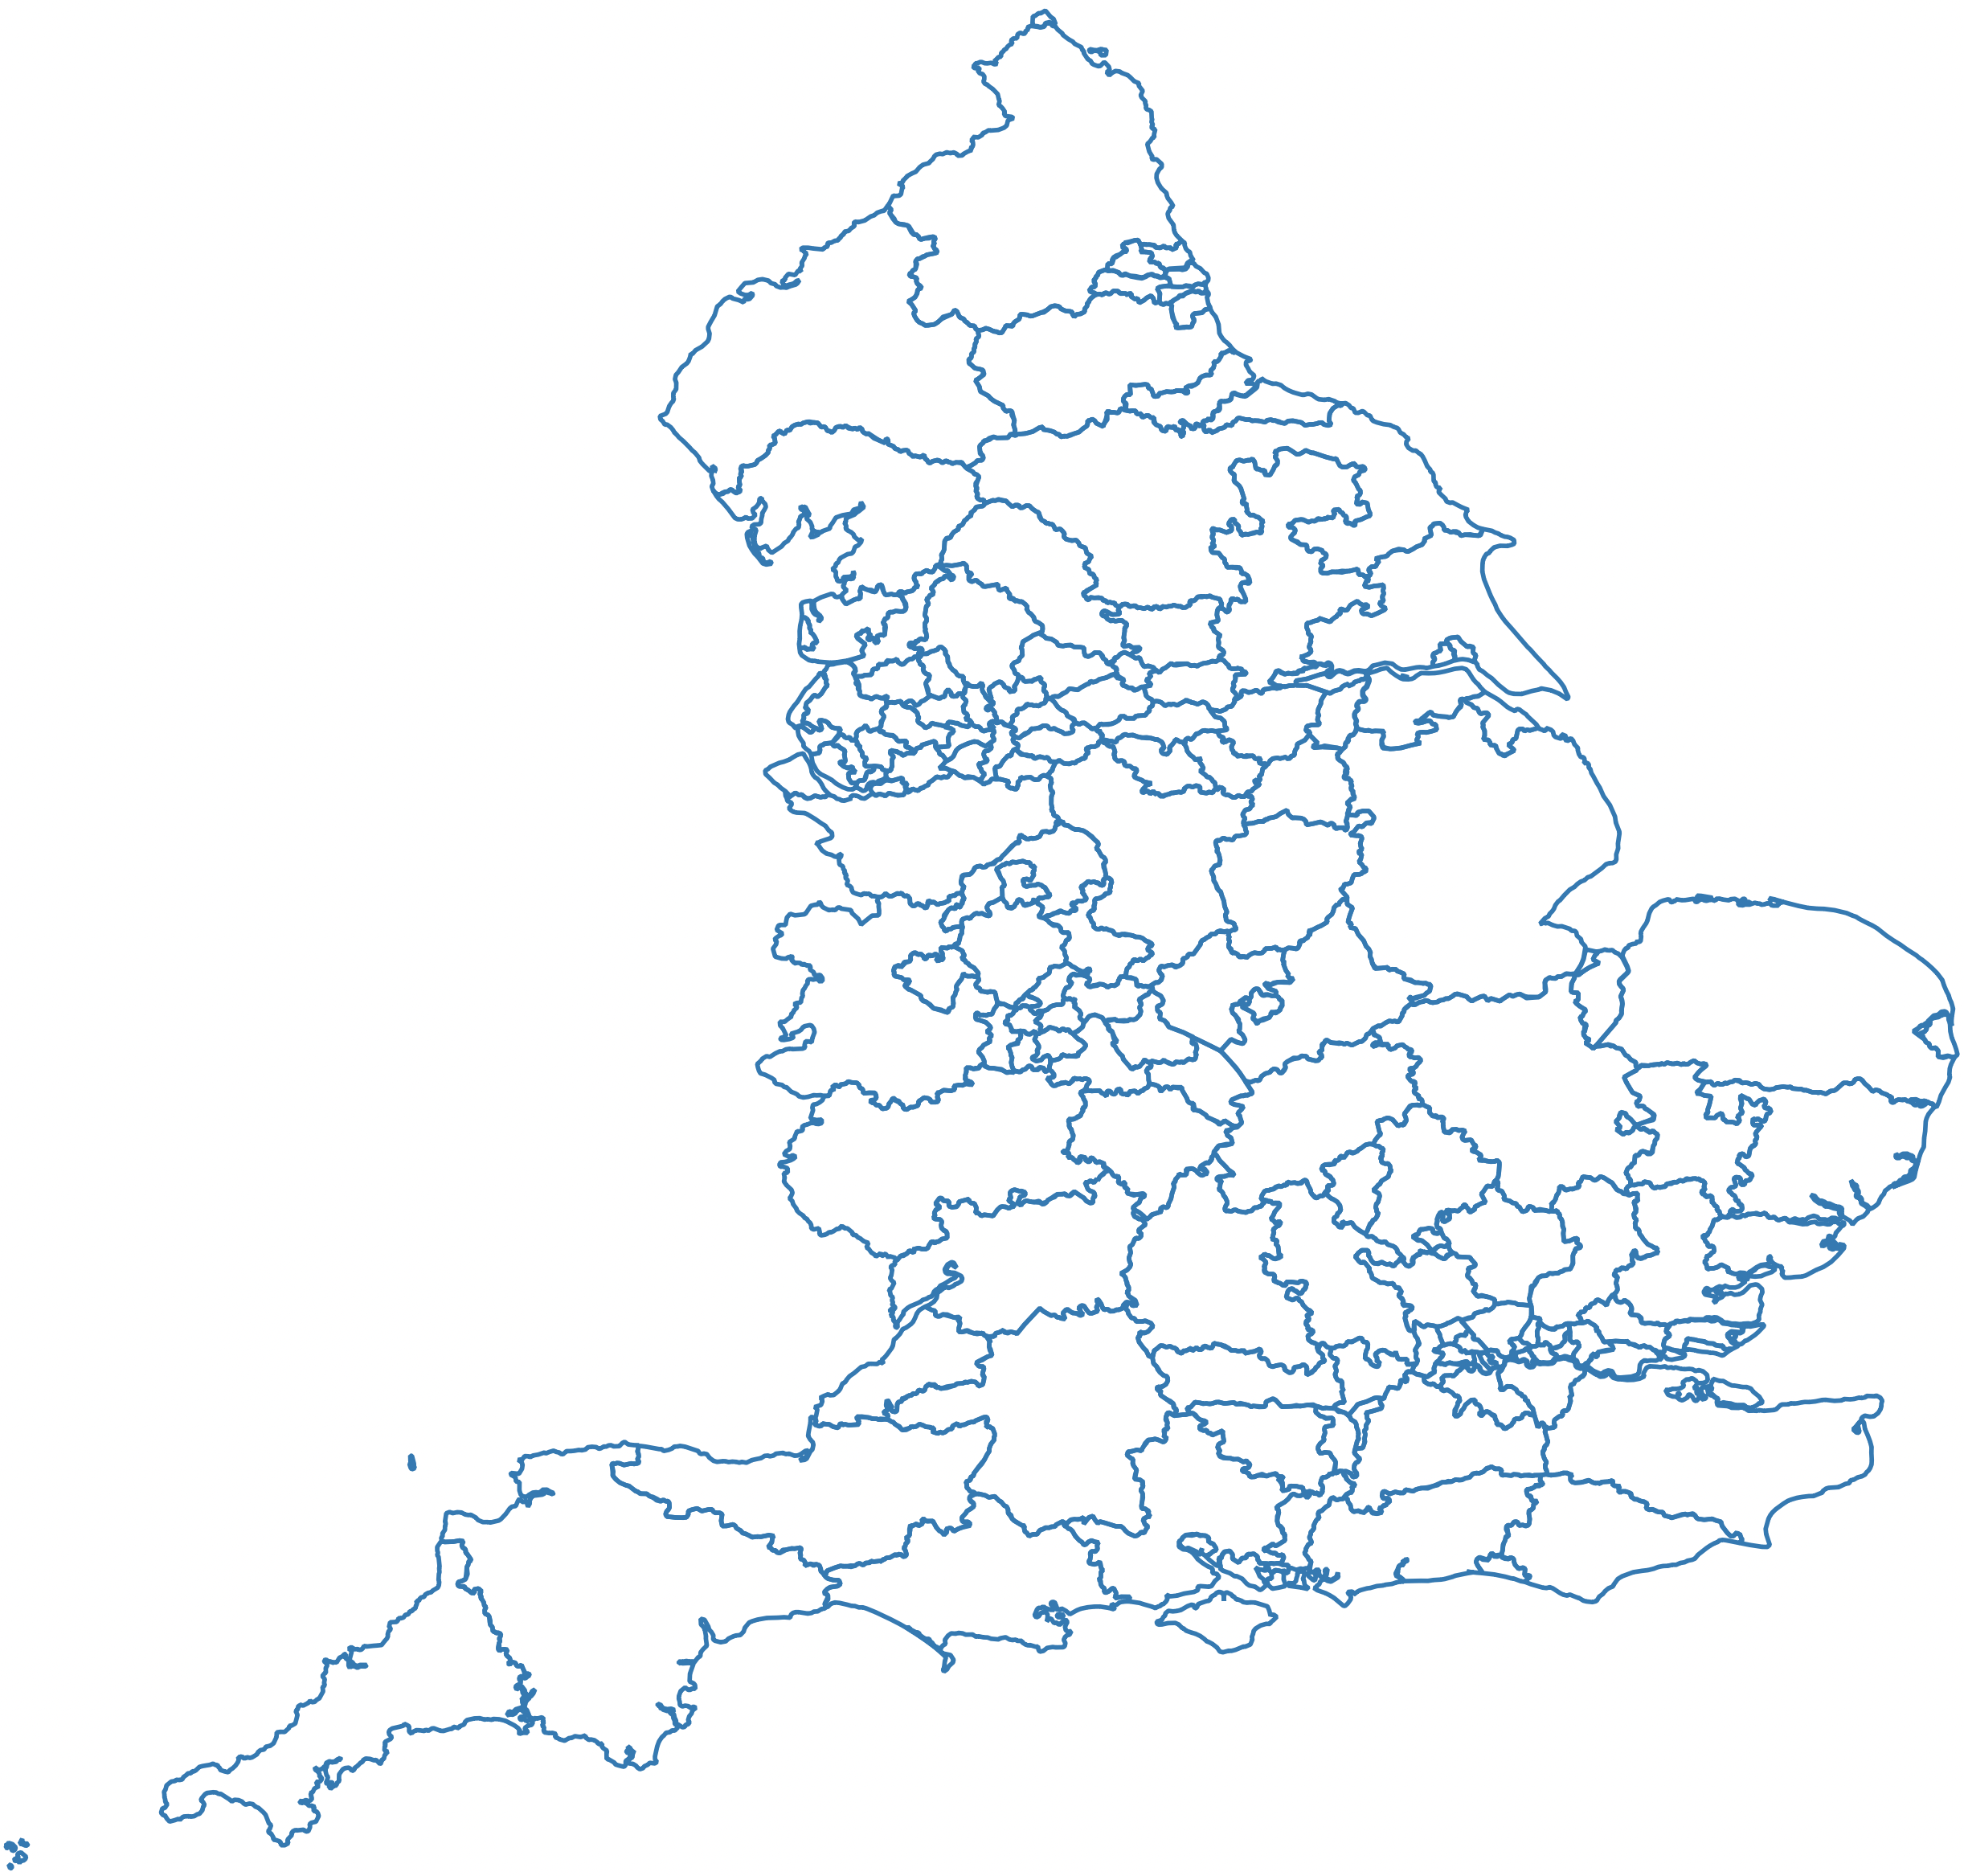
\includegraphics[width=0.6\columnwidth]{figure/ccg.png}
    \caption{A map of 135 CCGs in England as of 2020, obtained from the Open Geography portalx \cite{opengeographyportalxOpen}.}
    \label{fig:ccg}
\end{figure}
}

\subsubsection{Clinical Commissioning Groups Shapefile}

Clinical Commissioning Groups (CCGs) are the main geographic unit of the National Health Service (NHS) in the UK \cite{nhsNHS}. The number of CCGs changes over time due to the NHS re-organization. The most up-to-date shapefile is available from the Open Geography portalx \cite{opengeographyportalxOpen}. We decided to use the CCG shapefile from 2020 at the time of writing, because there is no public EHR data published based on the latest CCG re-organization that took place in 2021.

\subsubsection{River Features}

We used OpenStreetMap \cite{openstreetmapRelation} as our data source to obtain shapefiles for River Thames, River Trent and River Great Ouse in England. These rivers were chosen as they pass through regions with dense population, and provide informative geographical and topological cues. 

We first obtain a relation ID by searching for a river, e.g. River Thames, on OpenStreetMap. The relation ID is used to construct a query (See Listing~\ref{overpass}) which enables the user to download the entire river shapefile using Overpass Turbo \cite{overpassturboOverpass}.

\begin{lstlisting}[caption={The query that downloads the shapefile of River Thames from OpenStreetMap via the Overpass Turbo API.}, label={overpass},captionpos=b]
    relation(2263653);>>;
    out skel;
\end{lstlisting}

\subsection{EHR Data}

We obtained the Clinical Commissioning Group Outcomes Indicator Set (CCG OIS) from NHS Digital \cite{nhsdigitalClinical}. The OIS is a set of indicators that are used to measure the quality of care and the associated health outcomes in the NHS. Some datasets include:
\begin{itemize}
    \item Under 75 mortality
    \begin{multicols}{2}
        \begin{itemize}
            \item Cardiovascular disease
            \item Respiratory disease
            \item Liver disease
            \item Cancer
        \end{itemize}
    \end{multicols}
    \item Emergency hospital admission
        \begin{itemize}
            \item Stroke
            \item Alcohol-specific admission and readmission
            \item Coronary heart disease
            \item Readmissions within 30 days of discharge
            \item Children with lower respiratory tract infections
        \end{itemize}
\end{itemize}

For all datasets, a spreadsheet including the following data is provided:

\begin{itemize}
    \item Reporting period: Calendar year of registration
    \item Period of coverage: Start and end date or reporting period
    \item Breakdown: Organization type
    \item ONS code: UK Office for National Statistics CCG code
    \item Level: CCG Code
    \item Level description: CCG Name
    \item Gender
    \item Indicator value: Directly standardized mortality rate
    \item CI lower: lower 95\% confidence interval
    \item CI upper: upper 95\% confidence interval
    \item Denominator: The count of registered patients
    \item Numerator: Number of deaths
\end{itemize}

\section{Cartograms with Dynamic Features}

 {
  \begin{figure}[tb!]
      \centering
      \includegraphics[width=\columnwidth,keepaspectratio]{example-image-a}
      \caption{An screenshot of \software. Figure TBA.}
      \label{fig:overview}
  \end{figure}
 }

 {
  \begin{figure*}[tb!]
      \centering
      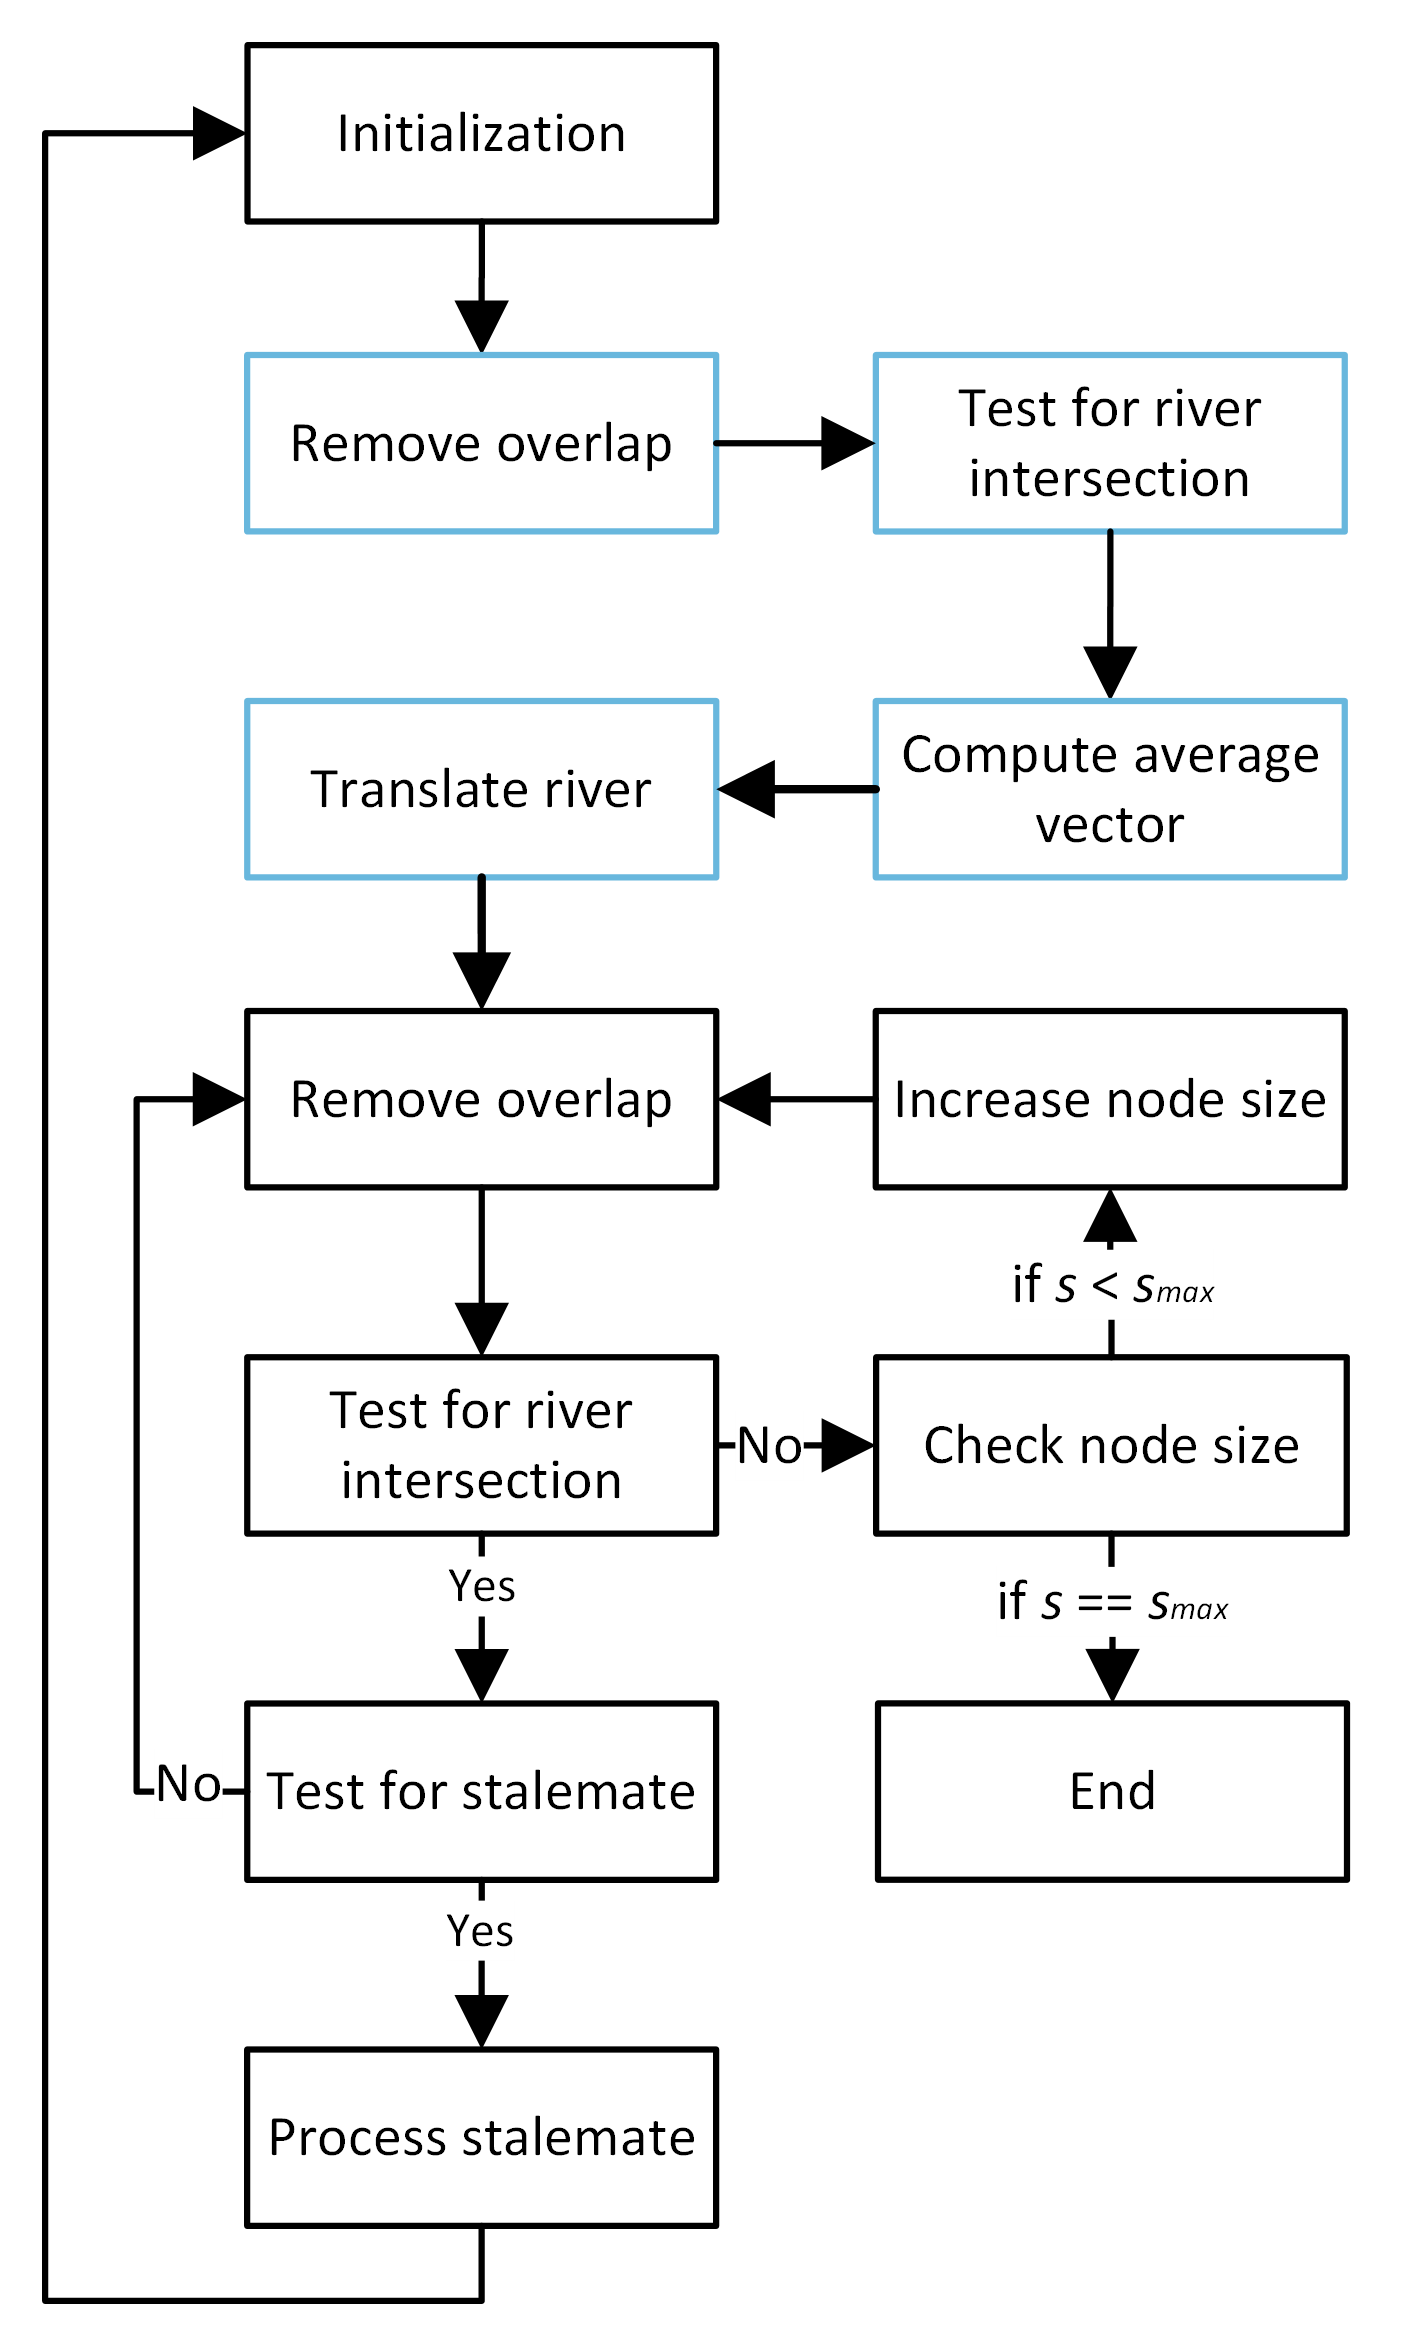
\includegraphics[width=\textwidth,height=0.95\textheight,keepaspectratio]{figure/flowchart.png}
      \caption{A flowchart illustration of our layout algorithm. See \autoref{fig:flowchart-stalemate} for the flow of processing stalemate. See also \autoref{alg:UpdateLayout} for more detail. For illustration purposes, we show the rendered views alongside the logical views representing the actual computation.}
      \label{fig:flowchart}
  \end{figure*}

  \begin{figure}[tb!]
      \centering
      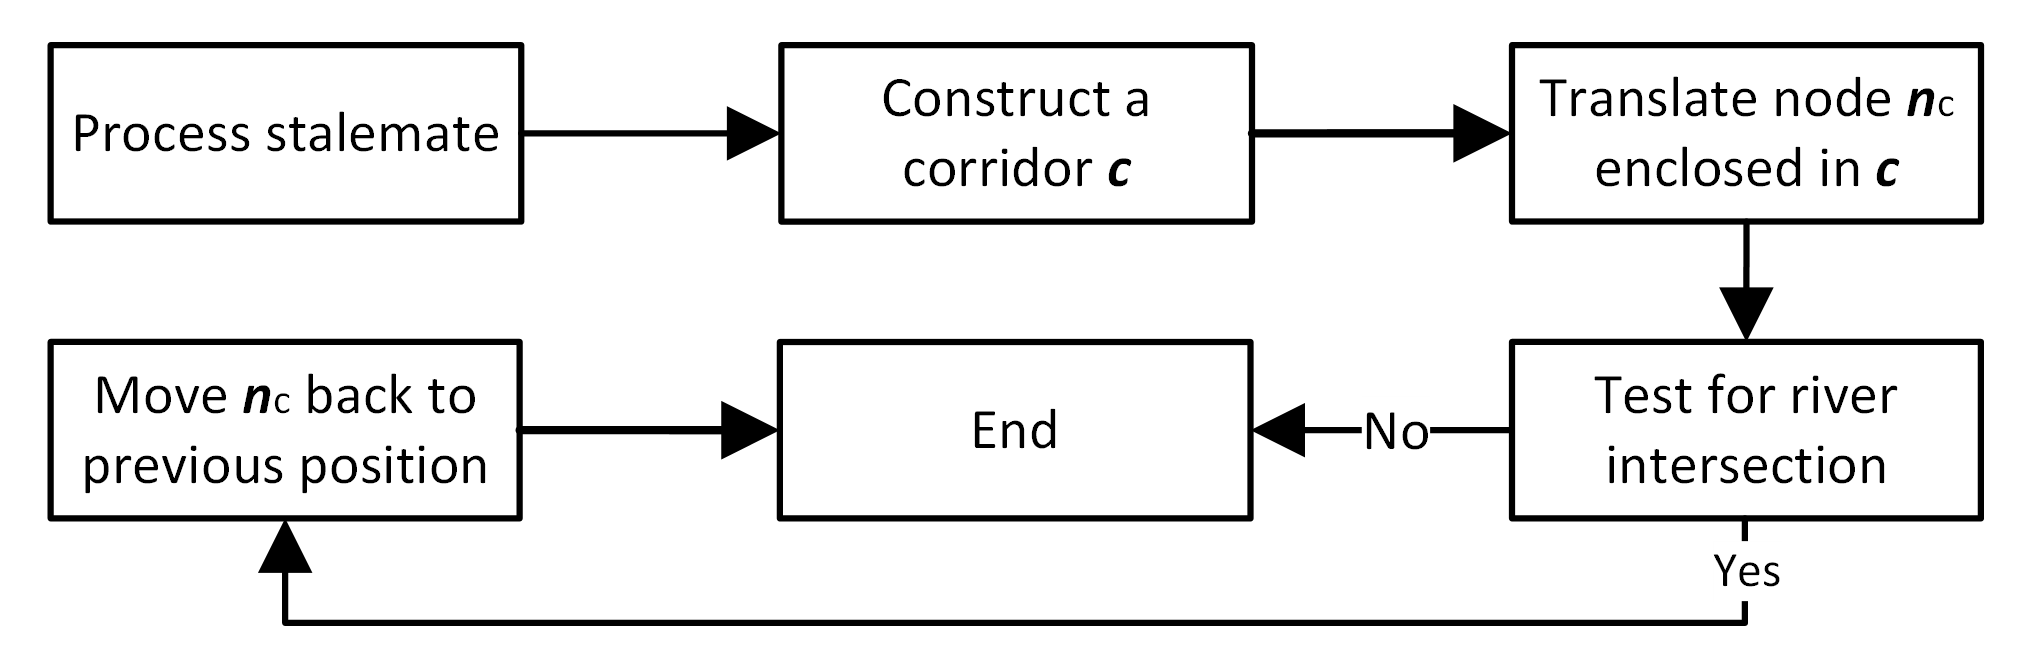
\includegraphics[width=0.9\columnwidth,keepaspectratio]{figure/flowchart stalemate.png}
      \caption{A flowchart illustration of stalemate processing.}
      \label{fig:flowchart-stalemate}
  \end{figure}
 }

\autoref{alg:UpdateLayout} and \autoref{fig:flowchart} provide an overview of the process.

\bobgraph{Initialization:} We first load and render the CCG geospatial boundaries. For each CCG we compute the centroid and represent it using a square node, $ \node $, with the initial size, $ \nodeSize $. We then load the river shapefiles and render the rivers. Since the vertices of the river in the shapefiles are not in sequential order, we first render the starting vertex, followed by the next closest vertex. This rendering approach enables us to adjust the river resolution as shown in \autoref{fig:river resolution}. We further apply a smoothing logic by removing vertices that are too close to each other.

\bobgraph{Node layout:} The basic algorithm is as follows: we first apply the Fast Node Overlap Removal (FNOR) algorithm that solves the Variable Placement with Separation Constraints (VPSC) problem \cite{dwyer2006fast} in order to remove overlaps. We chose FNOR over other node overlap removal algorithms because FNOR is able to provide spread minimization and node movement minimization while maintaining a good level of global shape preservation \cite{chen2020Node}. We gradually increase the node size by 1 unit at a time to ensure smooth transitions. An increase in $ \nodeSize $ can cause the nodes to overlap. During overlap removal, we compute node trajectories (See \autoref{alg:check river intersection}) and translate nodes to their new position. Nodes that cross a river are translated back to their previous position. If a node oscillates across a river, we process this as a stalemate. This procedure ends when 1) no node overlap is present; 2) no nodes cross a river. We then increase $ \nodeSize $ by one pixel and repeat the algorithm until the max node size $ \nodeSizeMax $ is reached. The gradual size increase process provides stability to the layout and helps minimize geographical error.



\begin{algorithm}[tb!]
    \caption{Procedure to adjust river positions, remove node overlap and prevent nodes from crossing rivers.}\label{alg:UpdateLayout}
    \textbf{Global variables:} \\
    $ \nodeList \gets $ a list of $ \node $ representing CCGs with the following properties: \\
    \-\hspace{1em}  \textcolor{blue}{$\nodeListCross \gets $ the number of $ \node $ in $ \nodeList $ that crosses a river} \\
    $ \nodeSize \gets $ the current size of all nodes \\
    $ \nodeSizeMax \gets $ the maximum size of a node \\
    \textcolor{blue}{ $ \riverList \gets $ a list of $ \river $ representing river features} \\
    $ \stalemateMax \gets $ the maximum number of iterations indicating a stalemate \\

    \textbf{Local variables:} \\
    $ \node \gets $ a node is an object with the following properties: \\
    \-\hspace{1em} $ \node.x, \node.y, $ or $ \node(x,y) \gets $ the x and y coordinates of $ \node $ \\
    \-\hspace{1em} $ \nodeCross \gets $ the counter for river crosses for $ \node $ \\
    \-\hspace{1em} $ \nodePrevious \gets $ the previous position of $ \node $ \\
    \-\hspace{1em} $ \nodeFNOR \gets $ the translated position of $ \node $ \\

    \begin{algorithmic}[1]
        \Procedure{UpdateLayout}{}
        \While{$ \nodeSize < \nodeSizeMax $}
            \State \textcolor{blue}{$ \nodeListCross \gets 1 $ \Comment{Trigger the while loop}}
            \While{$ \nodeListCross > 0 $}

                \State $ \nodeListCross \gets 0 $
                \State $ \nodeList \gets $ RemoveOverlap ($ \nodeList $)
                \color{blue}
                \State \Call{TranslateRiver}{$ \nodeList $}
                \State $\nodeListCross \gets $ \Call{TranslateNode}{$ \nodeList $}

                \color{black}

            \EndWhile

            \State $ \nodeSize \gets \nodeSize ++$

        \EndWhile

        \EndProcedure
    \end{algorithmic}
\end{algorithm}


\begin{algorithm}[tb!]
    \caption{Procedure to translate rivers.}\label{alg:TranslateRiver}
    \color{blue}
    \textbf{Input:} \\
    $ \nodeList \gets $ a list of $ \node $ representing CCGs \\

    \textbf{Local variables:} \\
    $ count \gets $ the number of river crossing nodes \\
    $ \node \gets $ a node is an object with the following properties: \\
    \-\hspace{1em} $ \node.x, \node.y, $ or $ \node(x,y) \gets $ the x and y coordinates of $ \node $ \\
    \-\hspace{1em} $ \nodeCross \gets $ the counter for river crosses for $ \node $ \\
    \-\hspace{1em} $ \nodePrevious \gets $ the previous position of $ \node $ \\
    \-\hspace{1em} $ \nodeFNOR \gets $ the translated position of $ \node $ \\

    \begin{algorithmic}[1]
        \Procedure{TranslateRiver}{$ \nodeList $}
        \ForEach {$ \river \in \riverList $}
        \State $ count \gets 0 $
        \State $ \riverVector \gets (0,0) $ \Comment{Hold the sum of vectors $ \nodeVectorCT $}
        \ForEach {$ \node \in \nodeList $}

        \If {$ \node(x,y) \neq \nodeFNOR(x,y) $}
        \If{ \Call{TestIntersection}{$ \nodeFNORLine $, $ \river $} $ = True $}
        \State $ \riverVector \gets \riverVector + \nodeVectorCT$
        \State $ count \gets count ++ $
        \EndIf

        \EndIf

        \EndFor

        \State Translate river $ \river $ by the average vector $ \frac{\riverVector}{count} $
        \EndFor

        \EndProcedure
    \end{algorithmic}
\end{algorithm}



\begin{algorithm}[tb!]
    \caption{Procedure to translate node positions.}\label{alg:TranslateNode}

    \color{blue}
    \textbf{Input:} \\
    $ \nodeList \gets $ a list of $ \node $ representing CCGs \\

    \textbf{Output:} \\
    $ count \gets $ the number of river crossing nodes in the input \\

    \textbf{Global variables:} \\
    $ \stalemateMax \gets $ the maximum number of iterations indicating a stalemate \\

    \textbf{Local variables:} \\
    $ \node \gets $ a node is an object with the following properties: \\
    \-\hspace{1em} $ \node.x, \node.y, $ or $ \node(x,y) \gets $ the x and y coordinates of $ \node $ \\
    \-\hspace{1em} $ \nodeCross \gets $ the counter for river crosses for $ \node $ \\
    \-\hspace{1em} $ \nodePrevious \gets $ the previous position of $ \node $ \\
    \-\hspace{1em} $ \nodeFNOR \gets $ the translated position of $ \node $ \\

    \begin{algorithmic}[1]
        \Procedure{TranslateNode}{$ \nodeList $}
        \State $ count \gets 0 $
        \ForEach {$ \node \in \nodeList $}

                    \If {$ \node(x,y) \neq \nodeFNOR(x,y) $}
                        
                        \State $ \node(x,y) \gets \nodeFNOR(x,y) $

                        \If{ \Call{TestIntersection}{$ \nodeFNORLine $} $ = True $}
                            \State $ \nodeCross \gets \nodeCross ++ $
                            \State $ count \gets count ++ $

                            \If{$ \nodeCross < \stalemateMax $}
                                \State \hskip-2em \Comment{Translate back to previous position}
                                \State $ \node(x,y) \gets \nodePrevious(x,y) $

                            \Else

                                \State \Call{ProcessStalemate}{$ \node, \nodeFNOR $}
                                \State $ \nodeCross \gets 0 $ \Comment{Reset counter}

                            \EndIf
                            
                        \EndIf

                    \EndIf

                \EndFor
        \State \Return{$ count $}
        \EndProcedure
    \end{algorithmic}
\end{algorithm}

\color{black}



\subsection{River Intersection Testing}

We use rivers as topological boundaries and prevent nodes from crossing them. The resolution of rivers can be adjusted by the user, as shown in \autoref{fig:river resolution}, the number of vertices is reduced from 10,170 to 30. A pixel-level river resolution is not required as Demers cartograms do not need to represent geography at this level of detail. Instead a resolution that matches the node size is used. Enabling river simplification reduces the number of edge intersection tests that need to be performed. When a node's position changes, we test if the node's trajectory intersects any segment of a river. See \autoref{alg:check river intersection}. A bounding box intersection test between the edge defined by node translation and river edges can be performed to reduce the number of edge intersection tests required.


    {
        \begin{figure}[tb!]
            \centering
            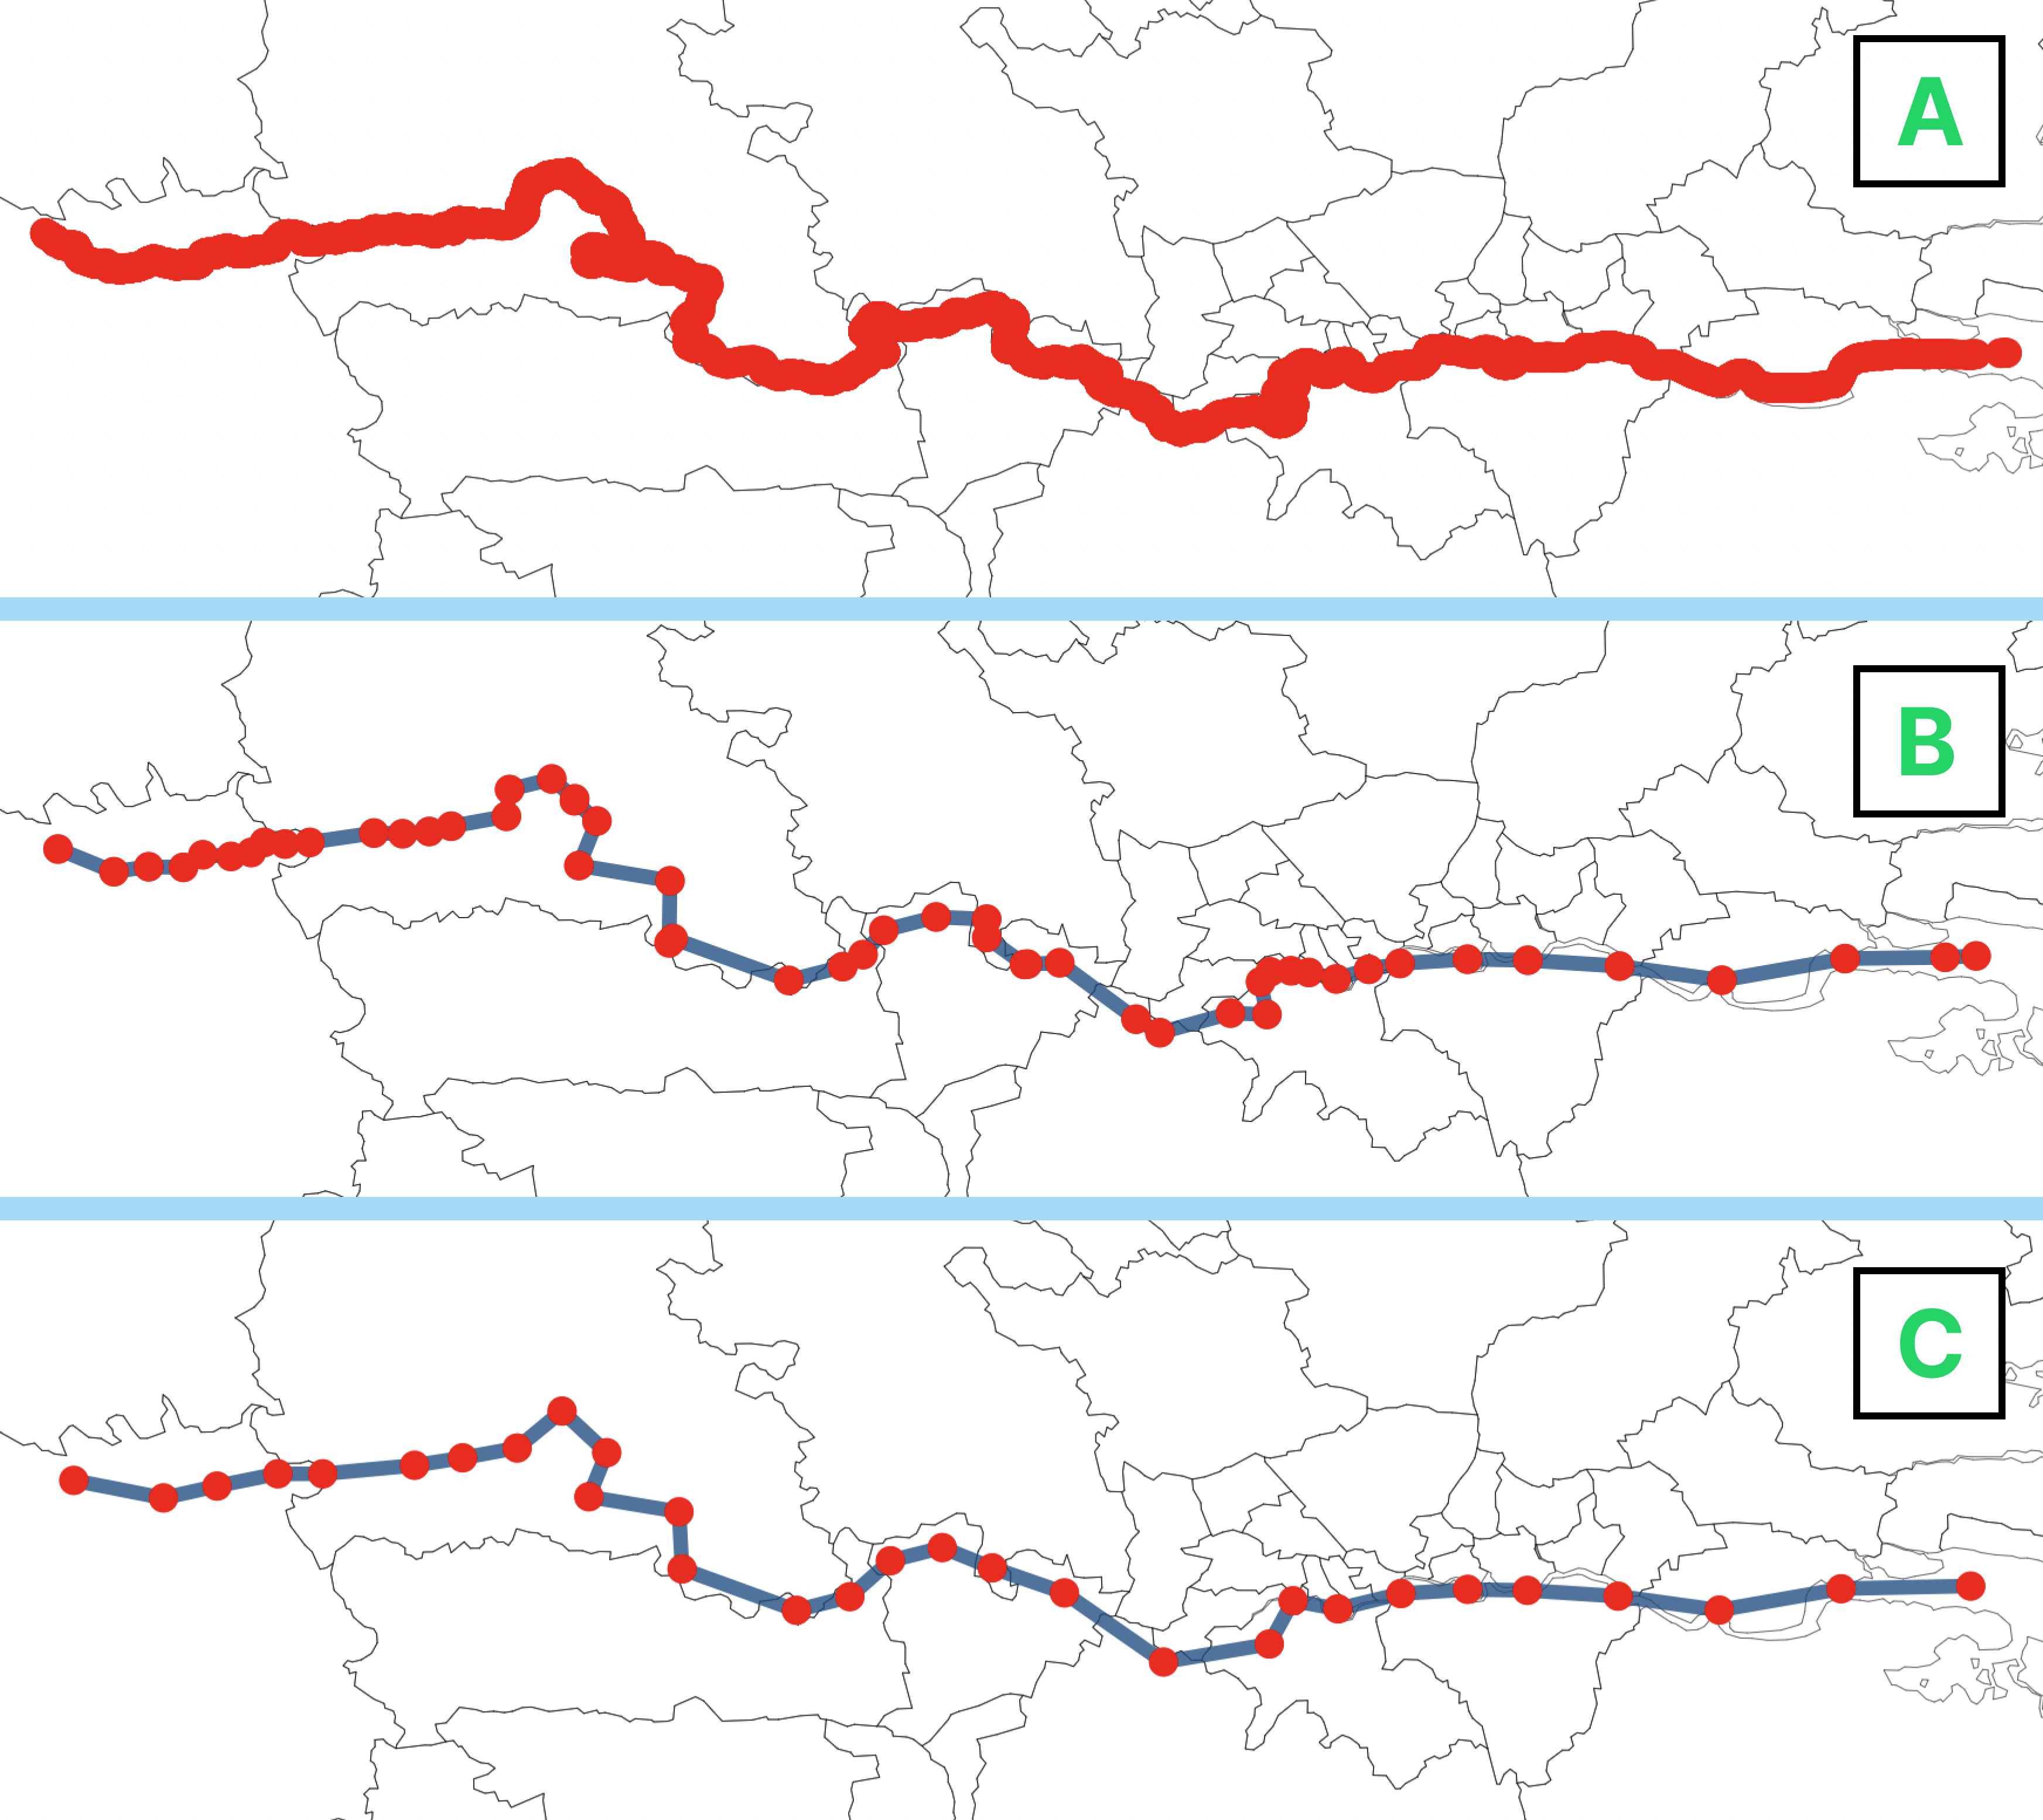
\includegraphics[width=\columnwidth,keepaspectratio]{figure/river_resolution.png}
            \caption{The resolution of rivers can be dynamically adjusted by the user. A shows River Thames at its original resolution with 10,170 edges. B shows the river at a reduced resolution of 49 edges. We further smooth the river by removing vertices in dense areas, as shown in C. The reduced resolution preserves the majority of River Thames' original shape and improves the performance of our river intersection tests.}
            \label{fig:river resolution}
        \end{figure}
    }

% \begin{noindent}
\begin{algorithm}[tb!]
    \caption{Procedure to test if a node's translation path, $ \nodeLineNV $ intersects a river.}\label{alg:check river intersection}
    \textbf{Input:} \\
    $ \nodeLineNV \gets $ the node's translation path \\
    $ \river \gets $ a river feature \\

    \textbf{Output:} \\
    Returns $ True $ if the node crosses a river. \\

    \textbf{Local variables:} \\
    $ \nodeBoundingBox, \riverEdgeBoundingBox \gets $ the bounding boxes for $ \nodeLineNV $ and $ \Edge $ \\
    $ \Edge \gets $ an edge of $ \river $ \\

    \begin{algorithmic}[1]
        \Procedure{TestIntersection}{$ \nodeLineNV $, $ \river $}
        
        \ForEach{$ \Edge \in \river $}
            \State $ \nodeBoundingBox \gets $ GetBoundingBox ($ \nodeLineNV $)
            \State $ \riverEdgeBoundingBox \gets $ GetBoundingBox ($ \Edge $)

            \If{$ \nodeBoundingBox ~intersect~ \riverEdgeBoundingBox = True $}
                \State \Return{$ \nodeLineNV ~intersect~ \Edge $}
                \EndIf
        \EndFor
        
        \State \Return{$ False $}
        \EndProcedure
    \end{algorithmic}
\end{algorithm}
%\end{noindent}

\subsection{Detecting Stalemates}

As the FNOR always attempts to produce an optimal node layout where node distribution and translation are minimized, a node's translation path can repeatedly intersect a river due to congestion, creating a stalemate situation, as shown in \autoref{fig:stalemate}. If a node is translated between two positions, $ \node $ and $ \nodeFNOR $, for $ \stalemateMax $ iterations (a user-adjustable parameter), we introduce a heuristic solution: constructing a corridor to alleviate the congestion. A corridor, $ \Corridor $, is a rectangle with a width of $ \CorridorWidth $ and a length of $ \CorridorLength $, formed by deriving two edges $ \EdgeParallelA $ and $ \EdgeParallelB $ such that $ \EdgeParallelA \parallel \EdgeParallelA \parallel \nodeLineNtNc $ (See \autoref{fig:corridor}C and D). All nodes enclosed by $ \Corridor $ are then translated by $ \nodeVectorTC $ to alleviate the congestion (See \autoref{fig:corridor}E).

    {
        \begin{figure}[tb!]
            \centering
            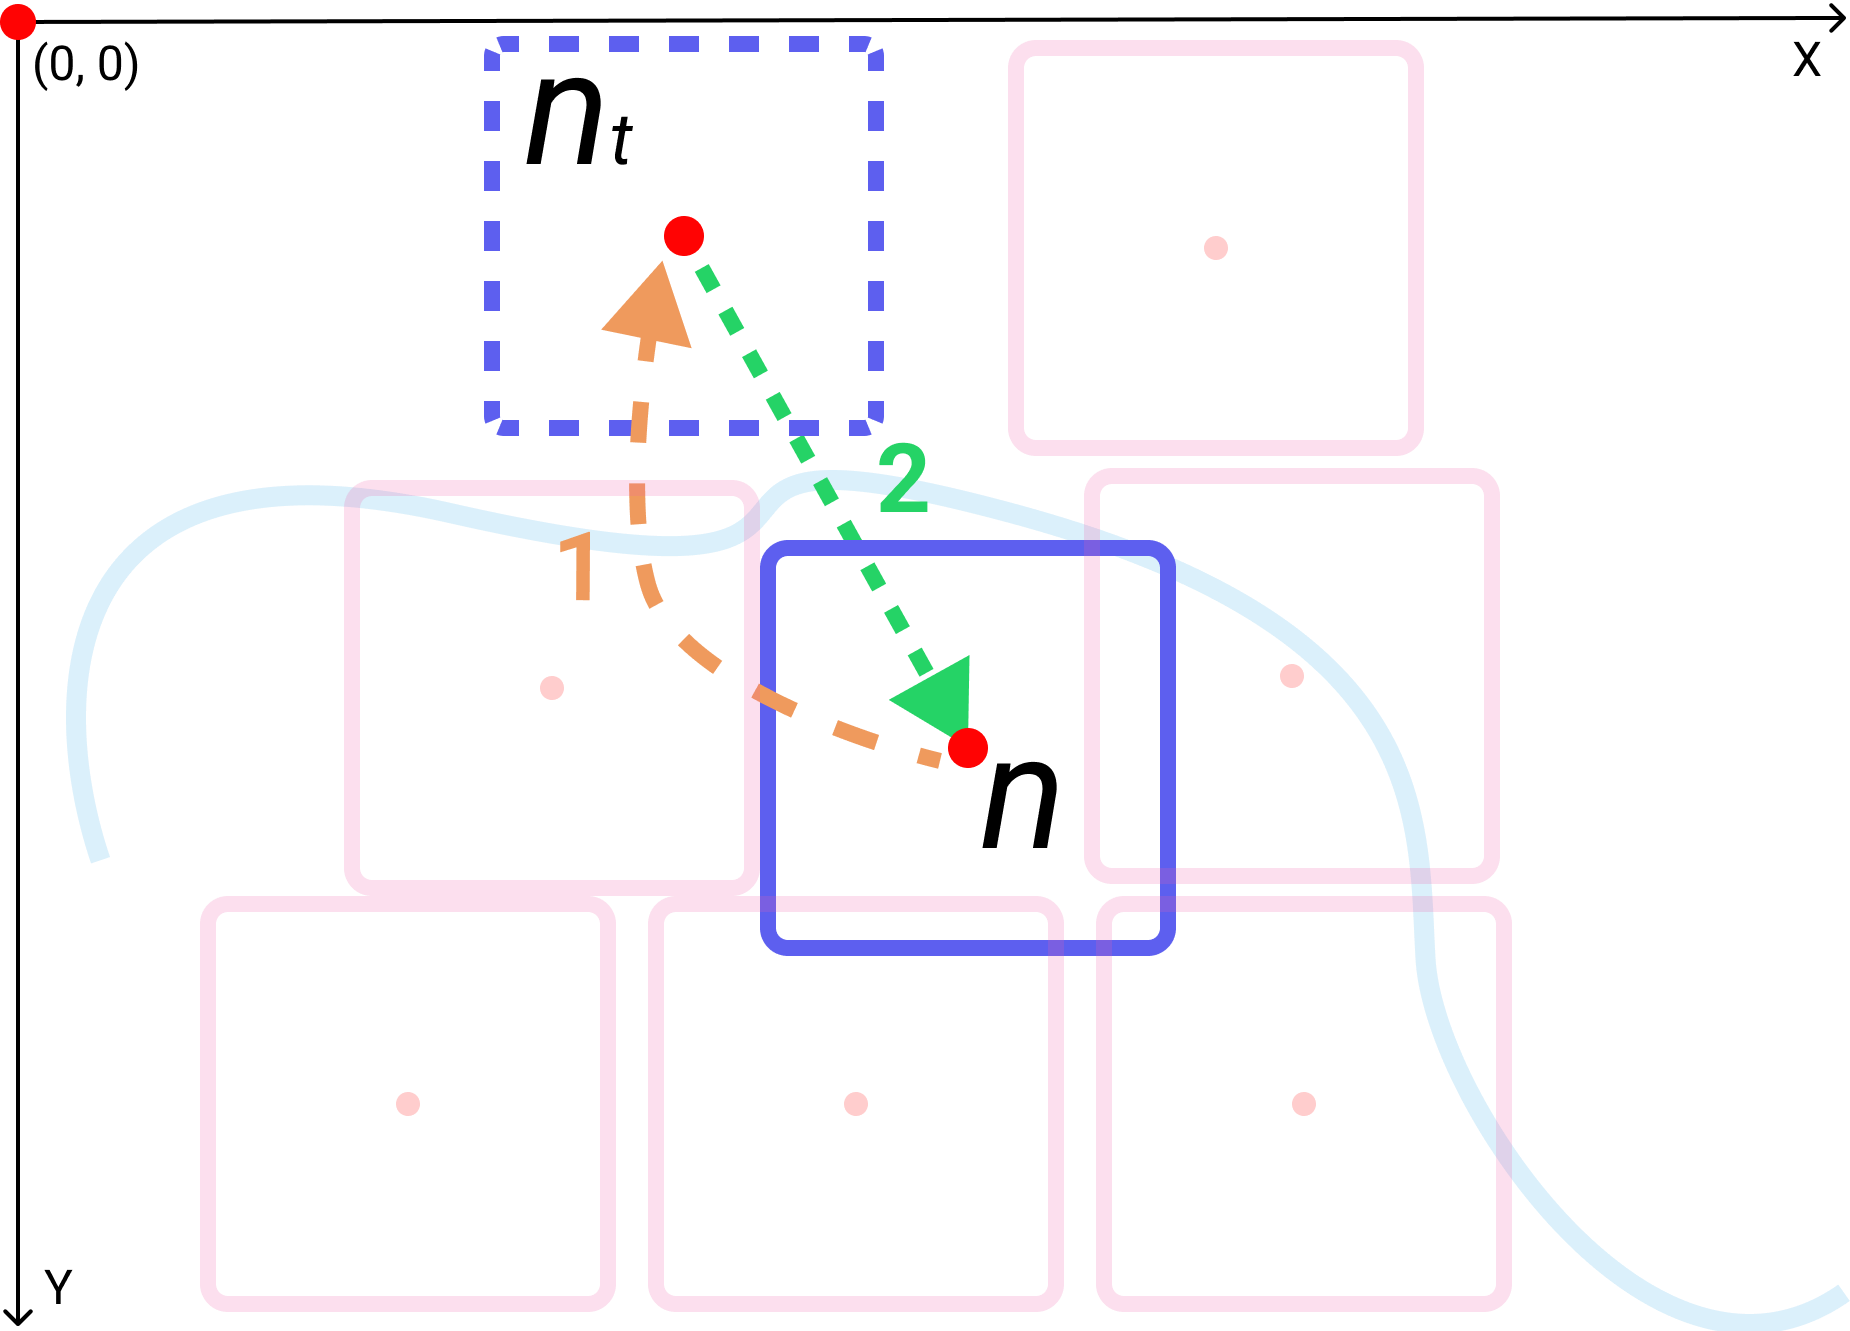
\includegraphics[width=\columnwidth,keepaspectratio]{figure/stalemate.png}
            \caption{A stalemate situation is when a node's translation path $ \nodeVectorCT $ (in iteration 1) intersects a river $ \stalemateMax $ times. The node is translated back to its previous position (iteration 2). A stalemate often occurs when the area is congested and the node is unable to translate to a new position without intersecting a river.}
            \label{fig:stalemate}
        \end{figure}
    }

    {
        \begin{figure}[tb!]
            \centering
            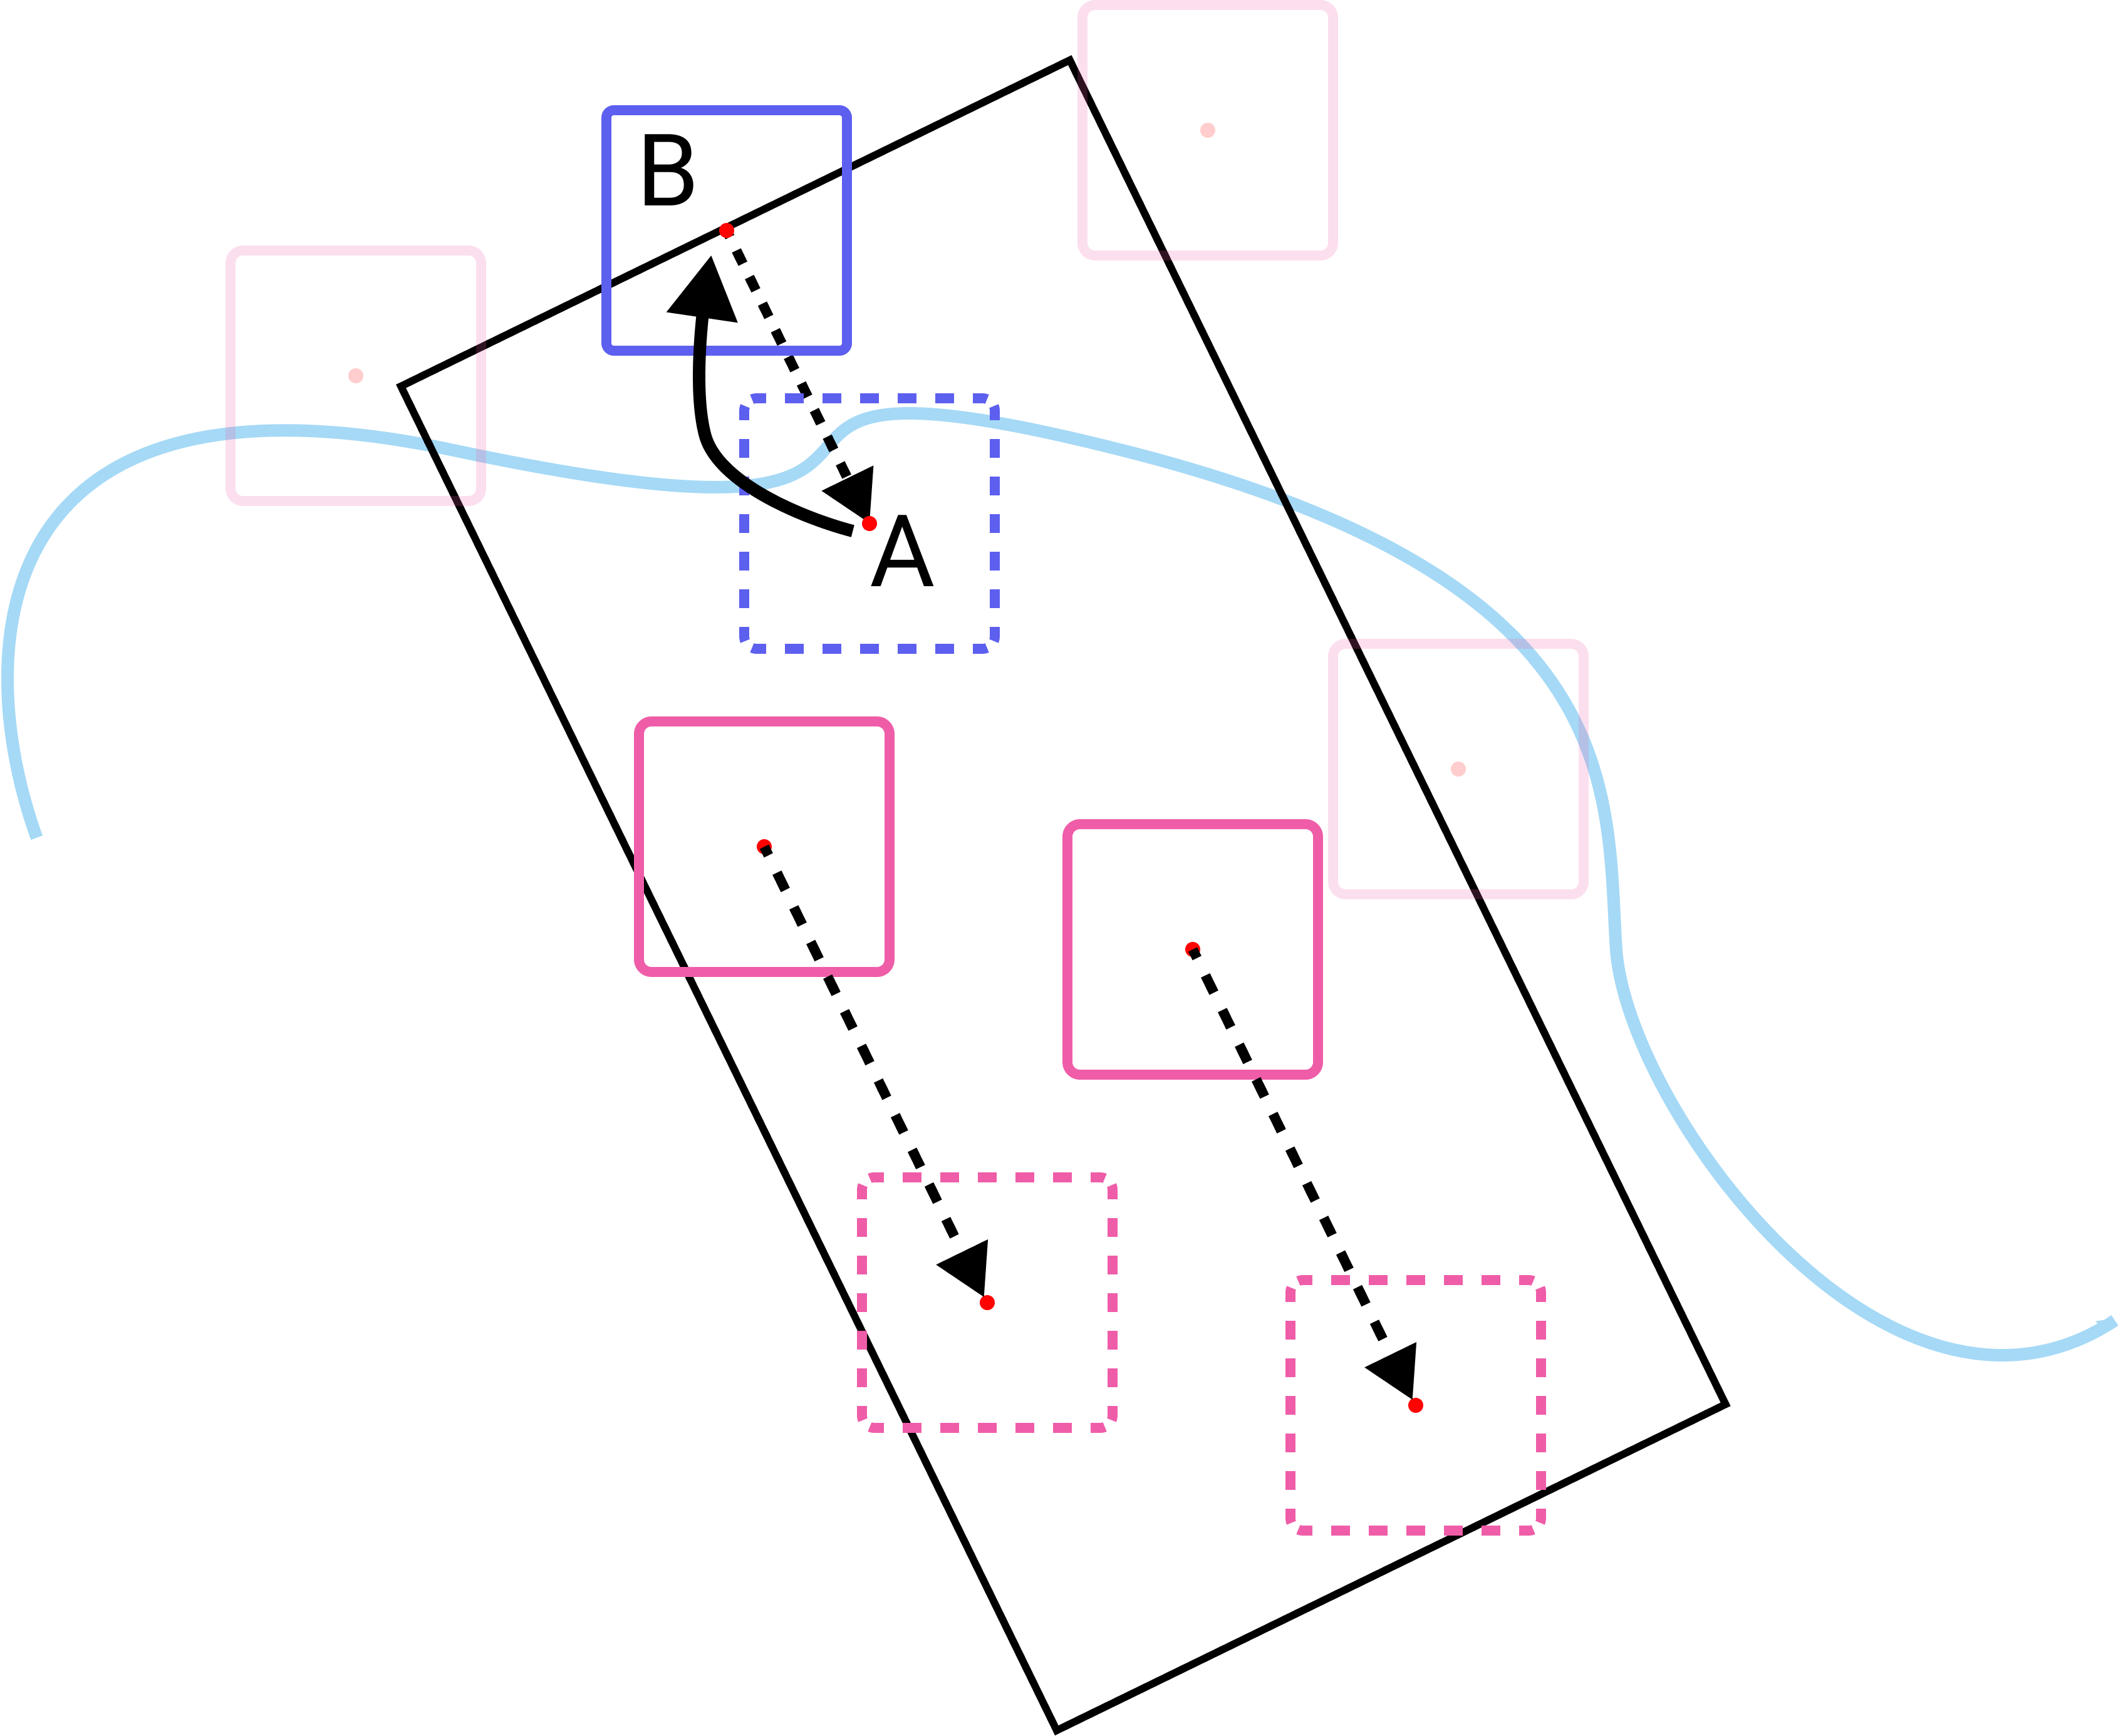
\includegraphics[width=\columnwidth,keepaspectratio]{figure/corridor.png}
            \caption{A stalemate occurs when a node's translation path $ \nodeVectorCT $ intersects a river for $ \stalemateMax $ times, as shown in A. To address the issue, we derive a corridor (orange rectangle in E) based on $ \node $ and $ \nodeFNOR $. All nodes within the corridor are translated based on $ \nodeVectorTC $, such that $ \nodeVectorNNn = \nodeVectorNinNinn $. In order to show a clear illustration, we place nodes sparsely in this figure.}
            \label{fig:corridor}
        \end{figure}
    }

% \begin{noindent}

\begin{algorithm}[tb!]
    \caption{Procedure to derive a corridor to translate enclosed nodes. We use an SVG canvas, where the point of origin (0,0) is located at the top left corner, with the x-axis extending to the right and the y-axis extending downwards (See \autoref{fig:stalemate}).}\label{alg:derive corridor}

    \textbf{Input:} \\
    $ \node \gets $ the node used to derive the corridor \\

    \textbf{Global variables:} \\
    $ \CorridorLength \gets $ the length of a corridor \\
    $ \CorridorWidth \gets $ the width of a corridor \\

    \textbf{Local variables:} \\
    $ \Corridor \gets $ the corridor \\
    $ \PointP \gets $ the point extending $ \nodeVectorTC $ such that $ \nodeLineWidthNtP = \CorridorLength $\\
    $ \EdgeParallelA, \EdgeParallelB \gets $ the edges parallel to $ \nodeLineNtNc $ \\
    $ corridor \gets $ a rectangle formed by $ \EdgeParallelA $ and $ \EdgeParallelB $ \\

    \begin{algorithmic}[1]
        \Procedure{ProcessStalemate}{$ \node $}
            \State $ \node(x,y) \gets \nodePrevious(x,y) $

            \State $ \PointP \gets $ \Call{DerivePoint}{$ \nodeVectorTC $, $ \CorridorLength $}

            \State $ \EdgeParallelA \gets $ \Call{DeriveParallelEdge}{$ \nodeVectorNtP $, $ \frac{\CorridorWidth}{2} $}

            \State $ \EdgeParallelB \gets $ \Call{DeriveParallelEdge}{$ \nodeVectorNtP $, $ -\frac{\CorridorWidth}{2} $}

            \State $ \Corridor \gets
                \begin{bmatrix}
                    \EdgeParallelA.start &
                    \EdgeParallelA.end \\

                    \EdgeParallelB.start &
                    \EdgeParallelB.end \\
                \end{bmatrix} $

            \ForEach{$ \nodeInCorridor $ inside $ \Corridor $}

                \State $ \Vector{\nodeInCorridor ~\nodeInCorridorT} = \nodeVectorTC $

                \State $ \nodeInCorridor(x,y) \gets \nodeInCorridorT(x,y) $

            \EndFor
        \EndProcedure
    \end{algorithmic}
\end{algorithm}

%\end{noindent}


\section{Evaluation}

\section{Limitations and Future Work}

\section{Conclusions}

\section{Acknowledgments}
This work is funded by the grant EP/S010238/2 from the Engineering and Physical Sciences Research Council (EPSRC). EPSRC is a British Research Council that provides government funding for grants to undertake research and postgraduate degrees in engineering and the physical sciences.


\clearpage
% reset \section command for section title "References"
\let\section=\origsection
\printbibliography

\cleardoublepage

\appendix

\section{Pre-processing Shapefiles}
\label{app:pre-processing}
Shapefiles from different sources are likely to be incompatible. In our case, the NHS CCG shapefile is incompatible with the river shapefiles. The major reason for the incompatibility is the coordinate reference system (CRS). The CRS of the CCG shapefile is EPSG:27700 (OSGB36 - British National Grid). The CRS of the river shapefiles is EPSG:4326 (WGS84 - World Geodetic System). Here we provide some pre-processing steps using QGIS (version: 3.26.0-Buenos Aires) \cite{qgisWelcome} to handle the incompatibility issue and reduce shapefile size to improve performance.

\subsection{Import Shapefiles into QGIS}
We first load all three river shapefiles into QGIS \autoref{fig:import_rivers}, followed by the CCG shapefile \autoref{fig:import_ccgs}.

{
    \begin{figure}[tbh!]
        \centering
        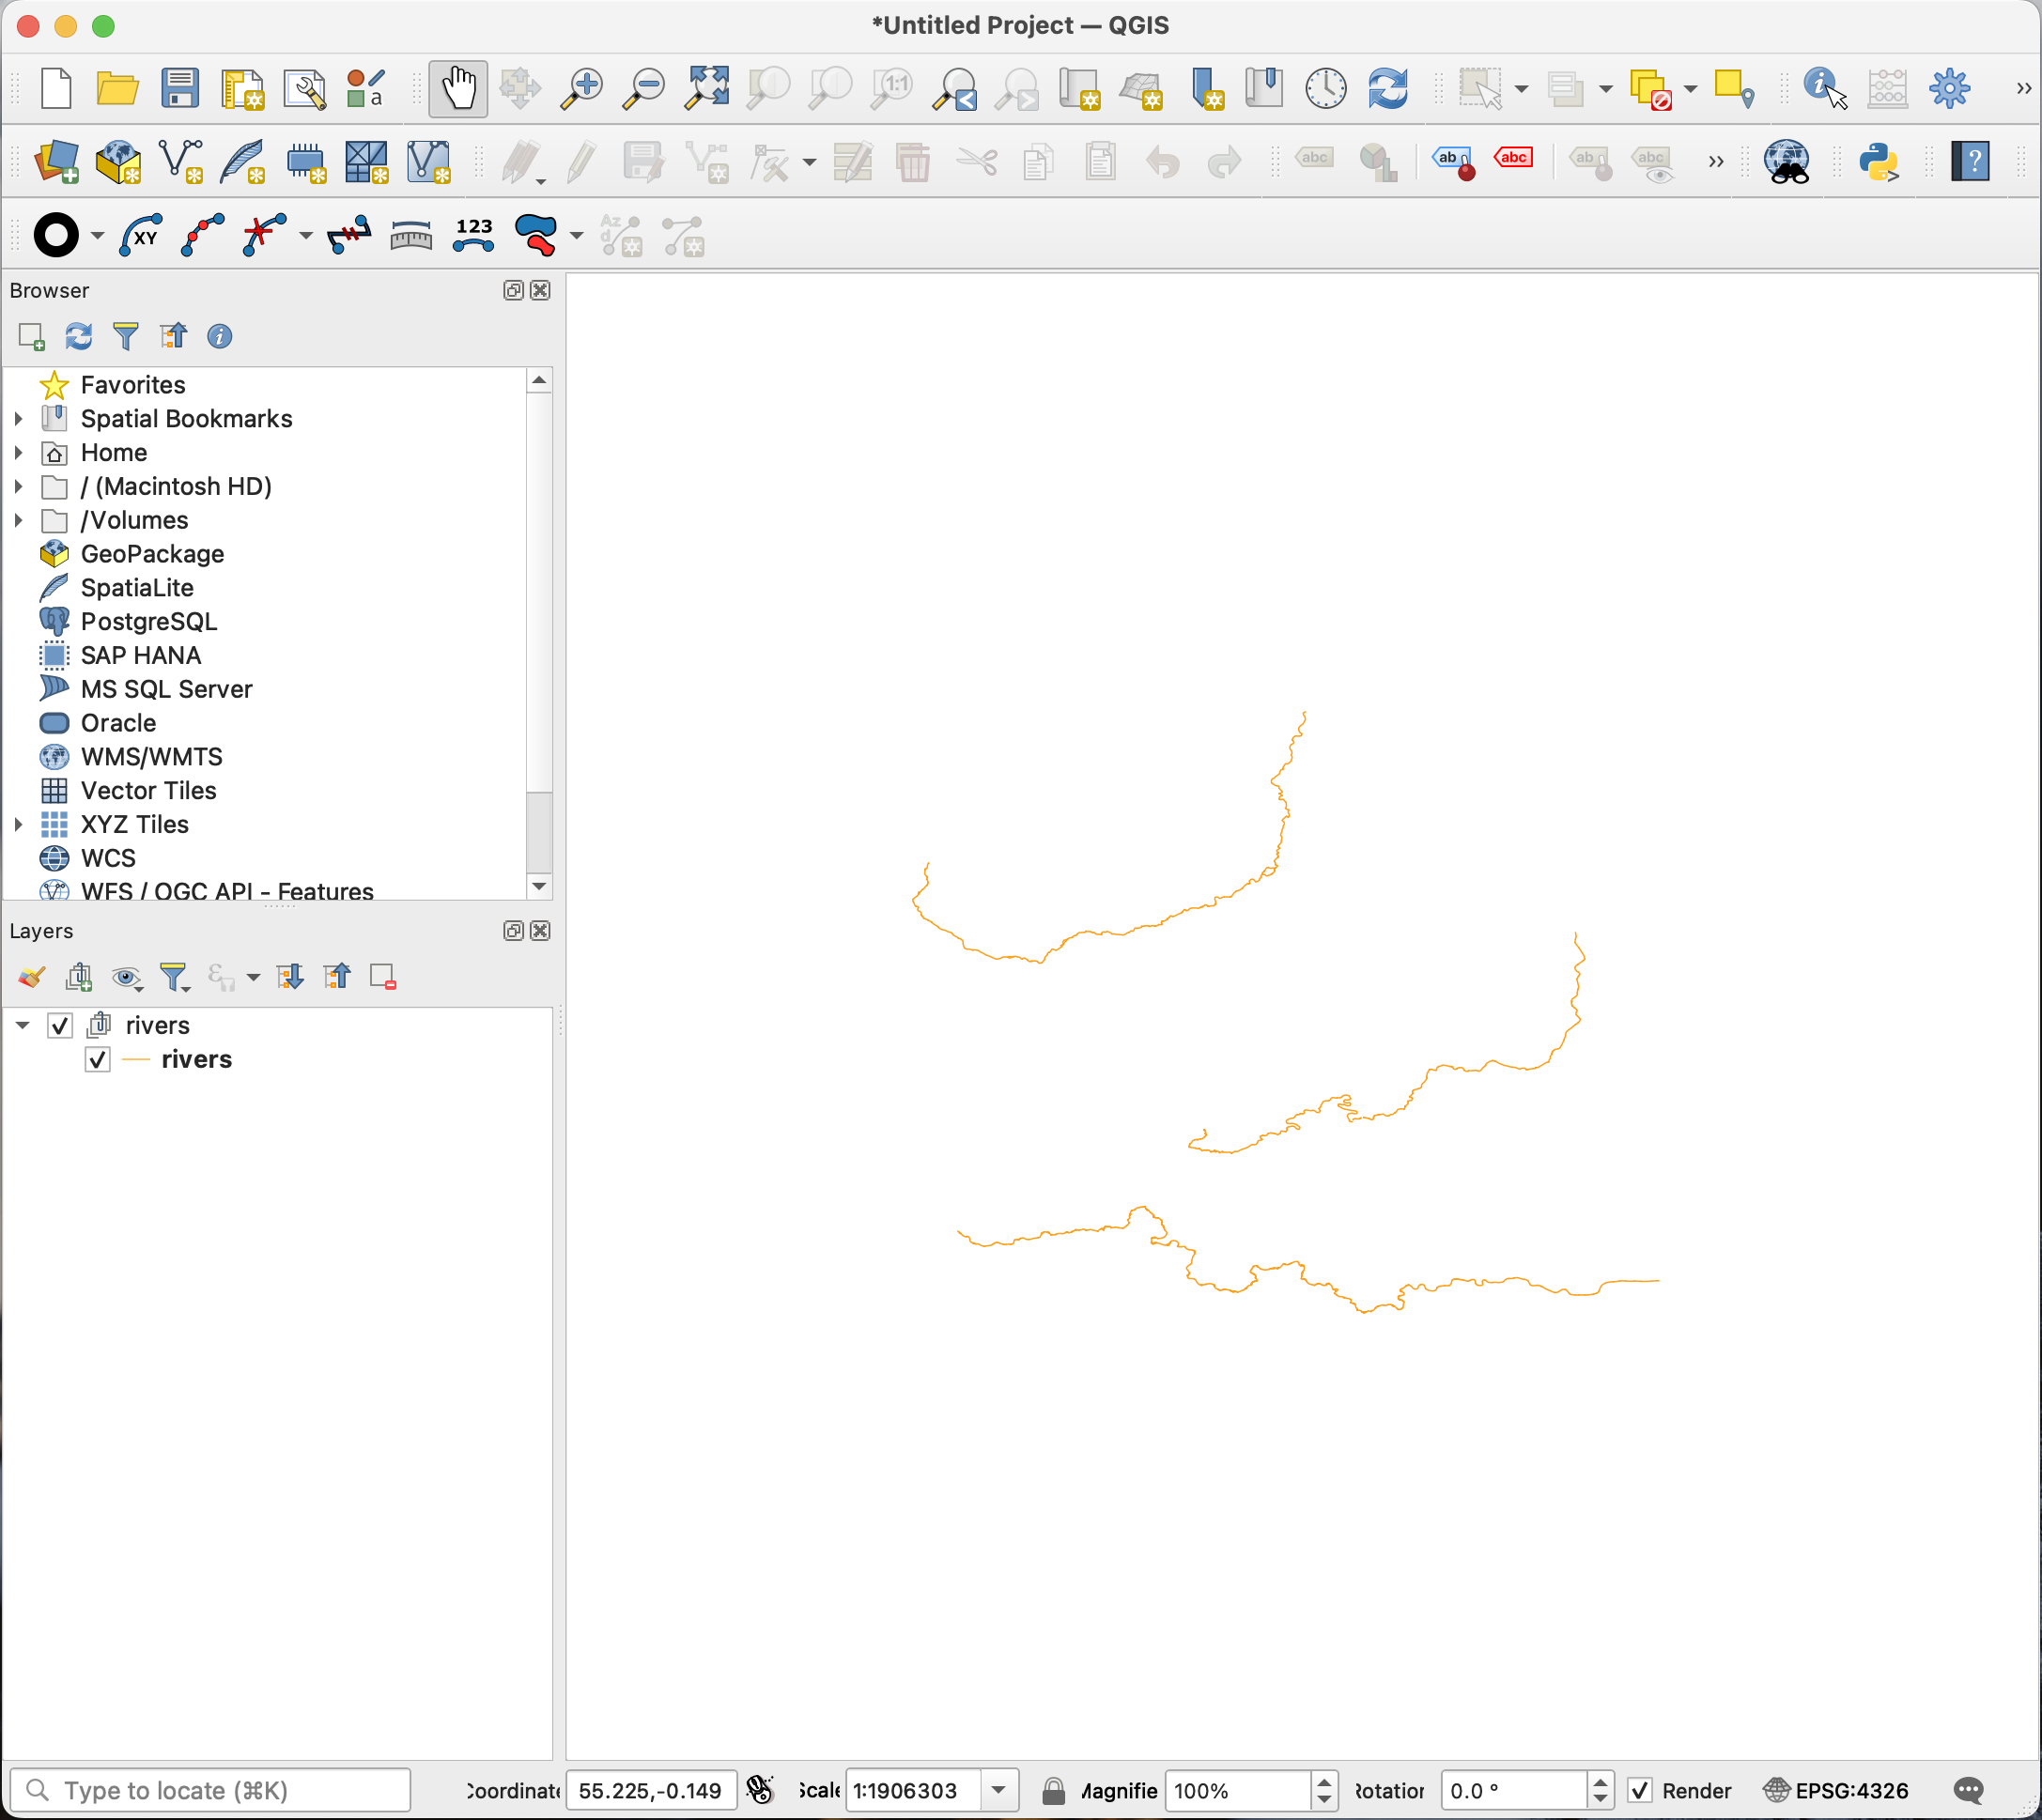
\includegraphics[width=\columnwidth]{figure/qgis/import_rivers.png}
        \caption{QGIS interface, with River Trent, River Great Ouse, and River Thames (from top to bottom) imported.}
        \label{fig:import_rivers}
    \end{figure}

    \begin{figure}[tbh!]
        \centering
        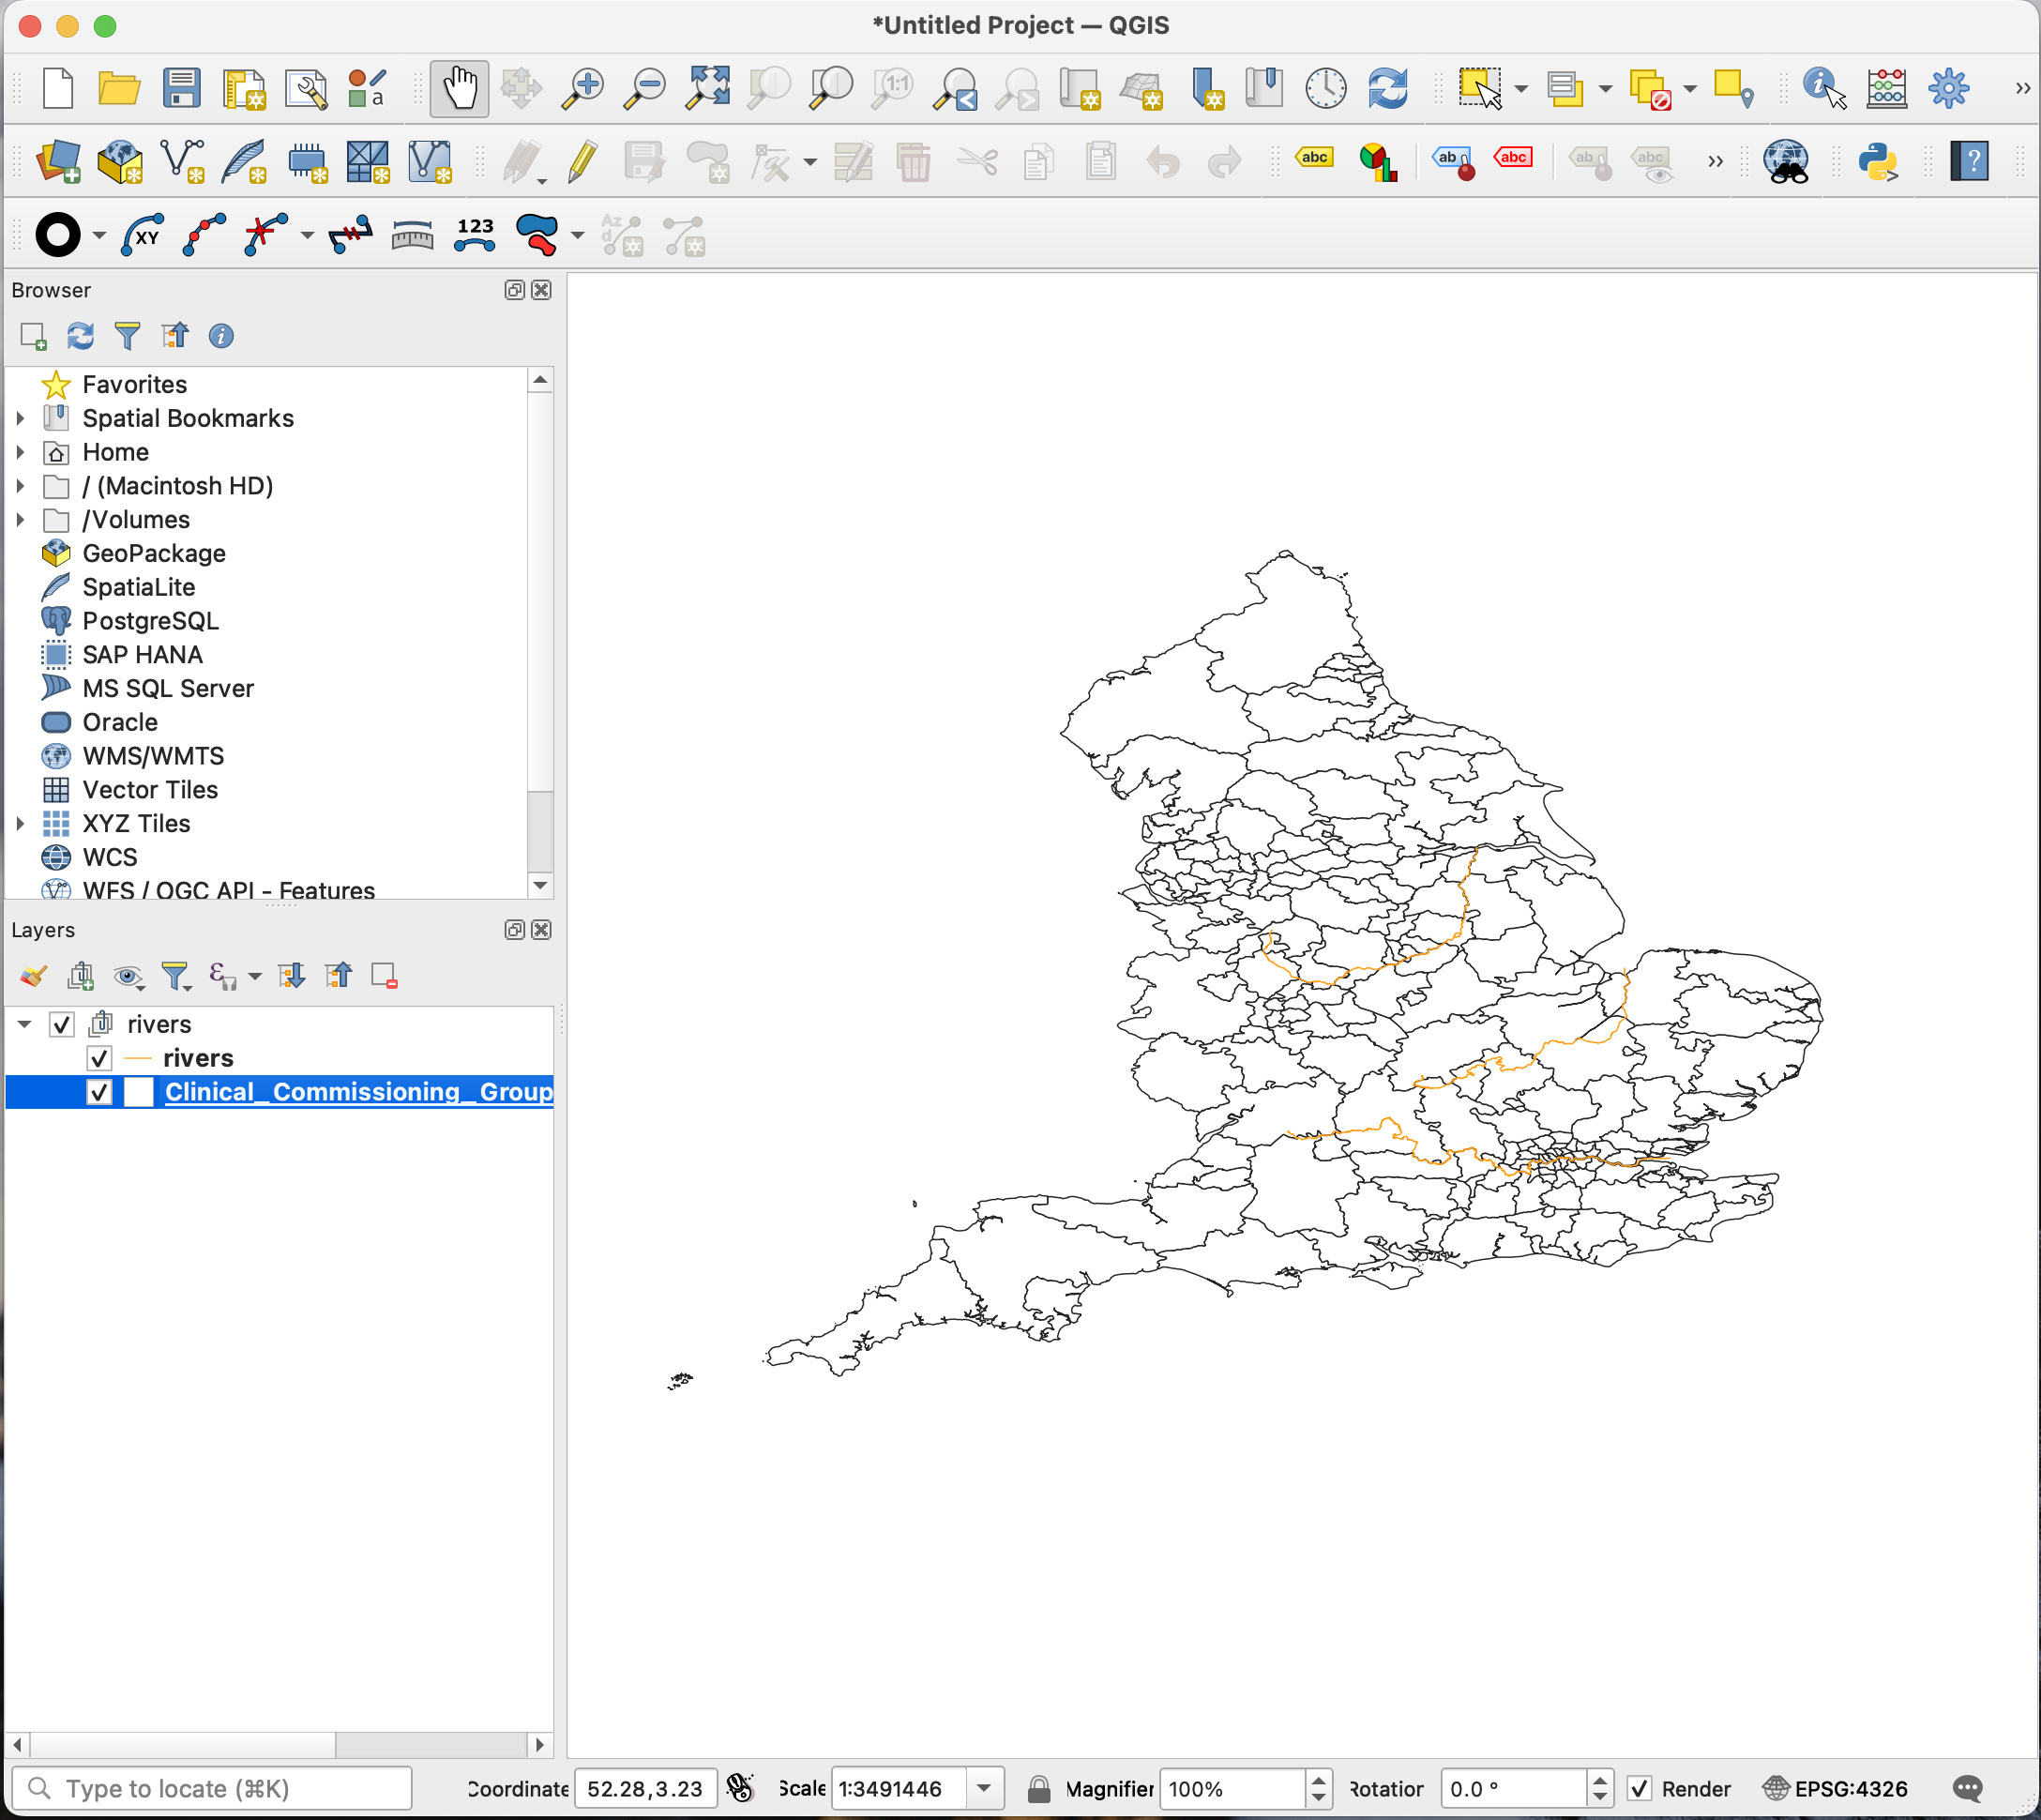
\includegraphics[width=\columnwidth]{figure/qgis/import_ccgs.png}
        \caption{QGIS interface, with all NHS CCGs imported.}
        \label{fig:import_ccgs}
    \end{figure}

    \begin{figure}[tbh!]
        \centering
        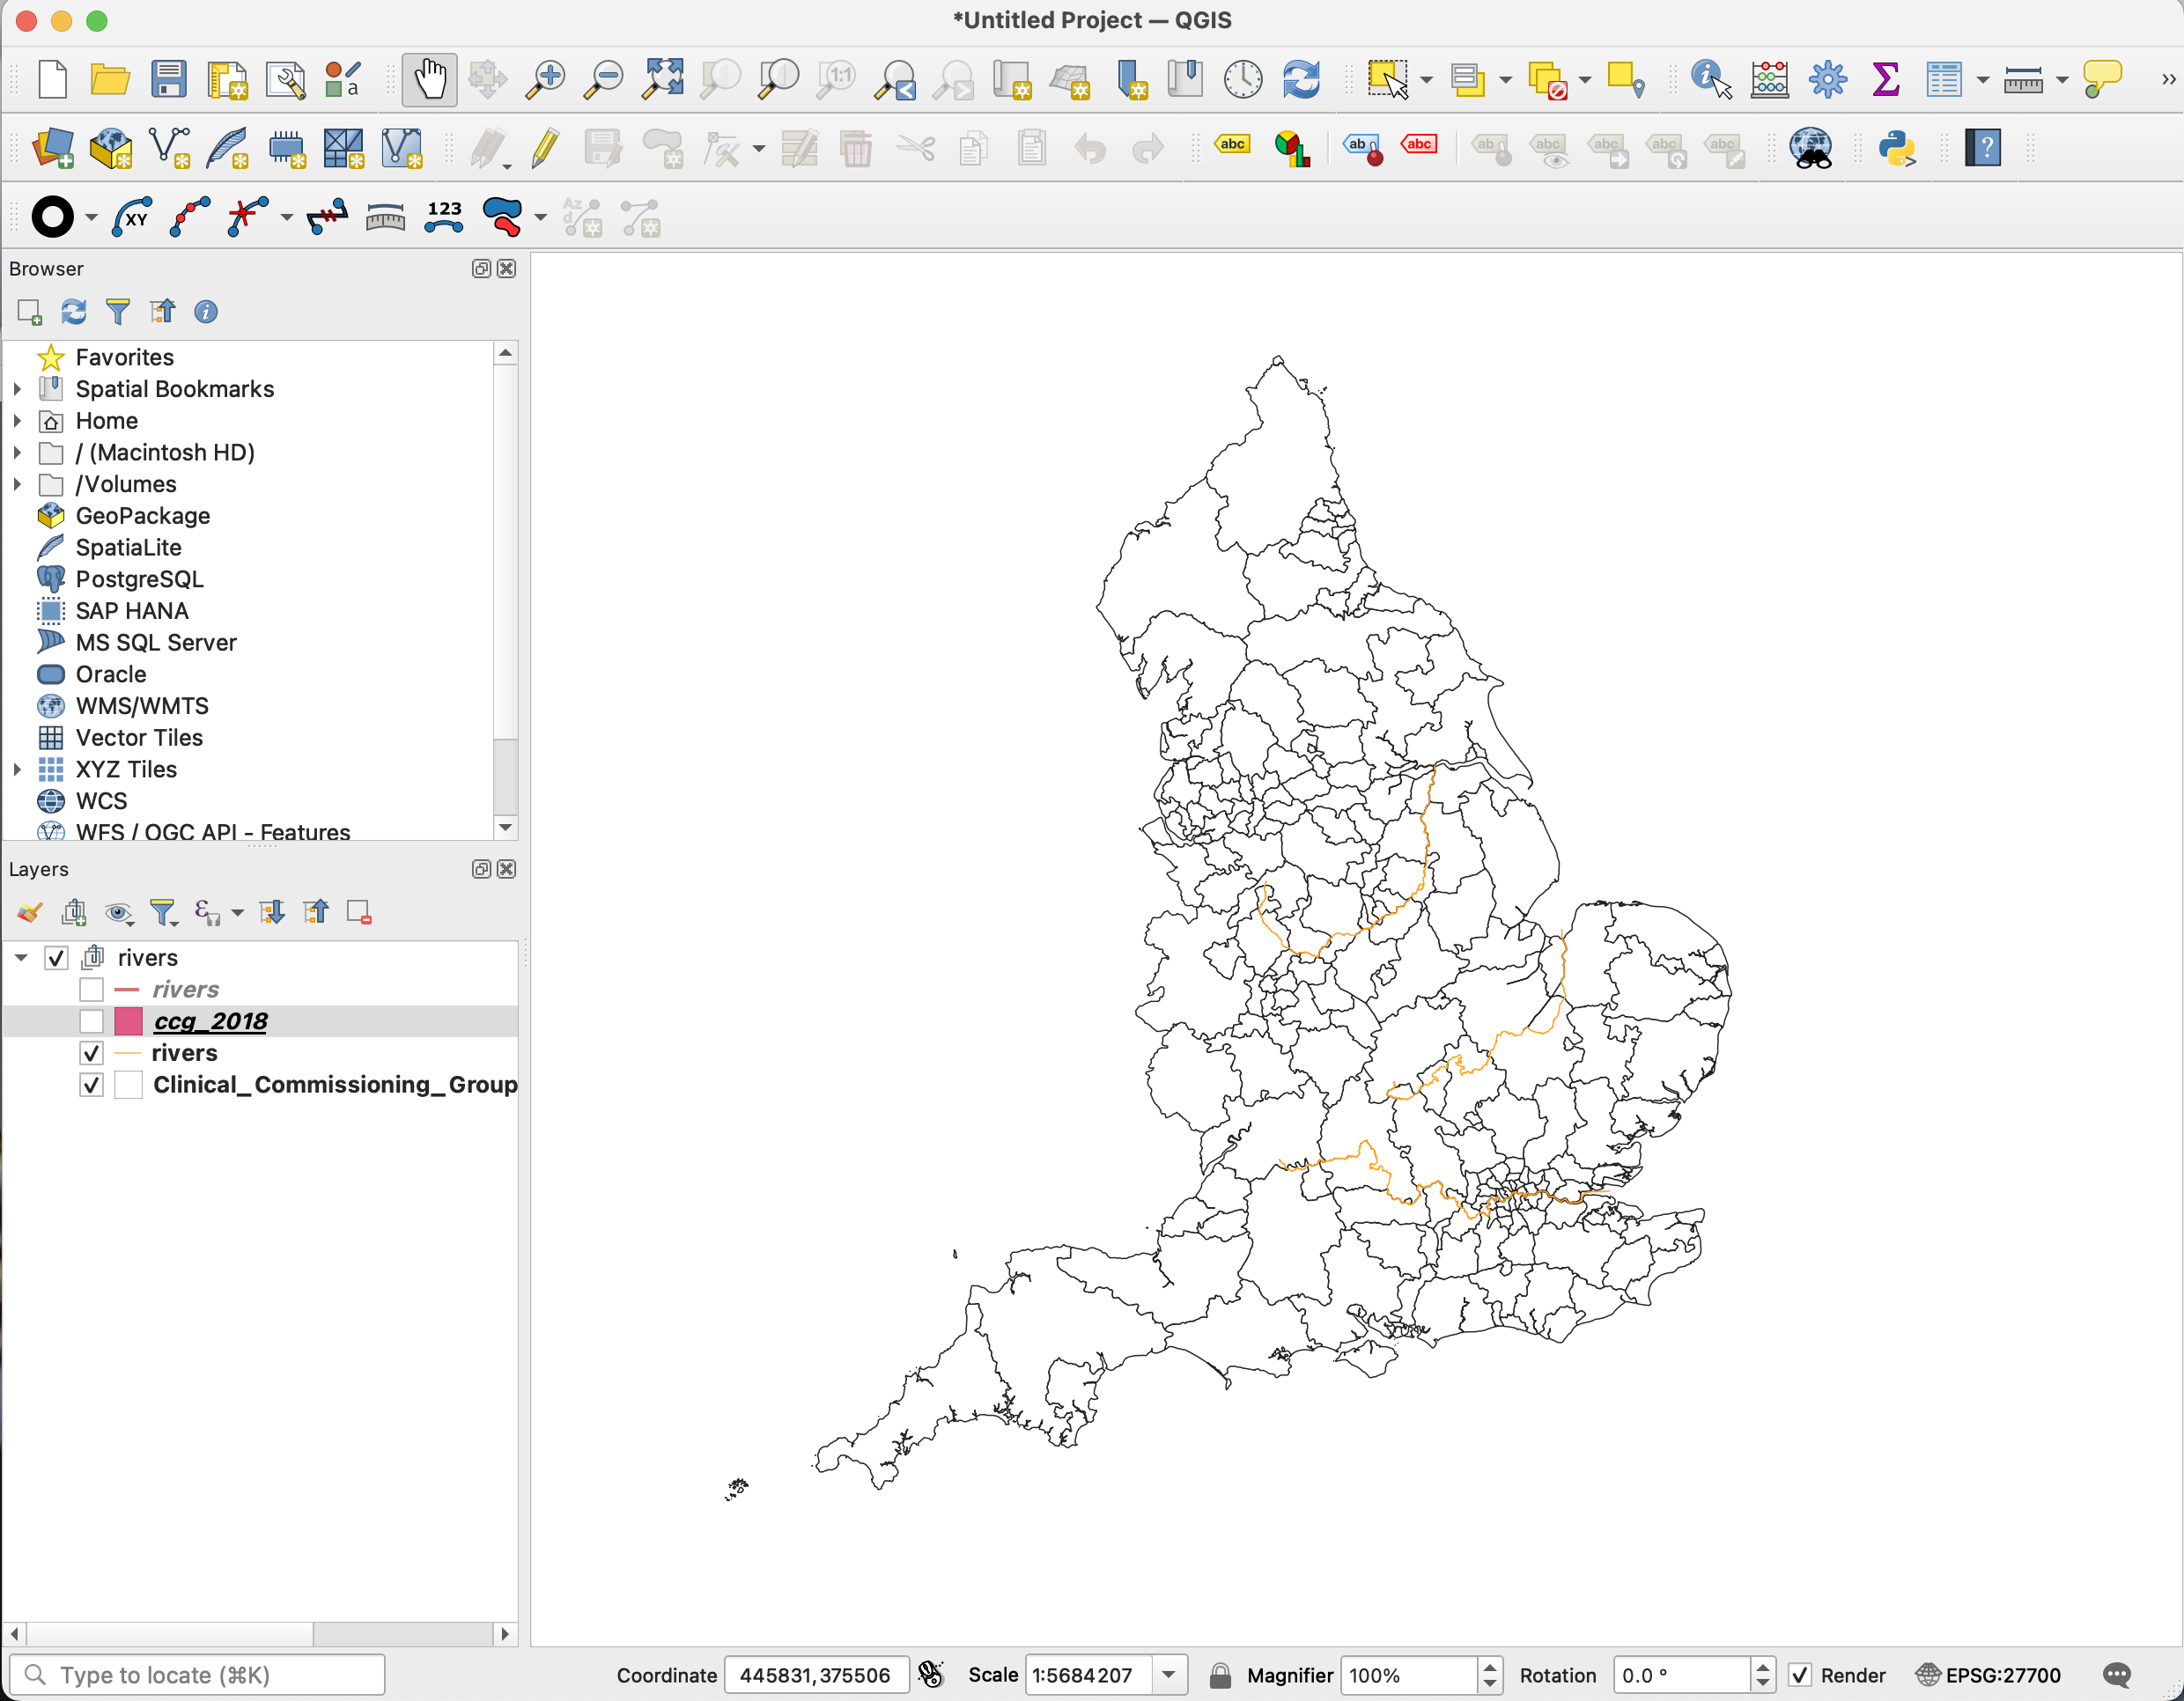
\includegraphics[width=\columnwidth]{figure/qgis/unify_crs.png}
        \caption{QGIS interface, showing the unified CRS (OSGB36) for both layers.}
        \label{fig:unify_crs}
    \end{figure}
}

\subsection{Export Shapefiles in GeoJSON and Unify the Coordinate Reference System (CRS)}

We then use QGIS to unify the CRS, and export both layers in the GeoJSON format. See \autoref{fig:export_rivers} and \autoref{fig:export_ccgs}. The unified layer is shown in \autoref{fig:unify_crs}.

{
    \begin{figure}[tbh!]
        \centering
        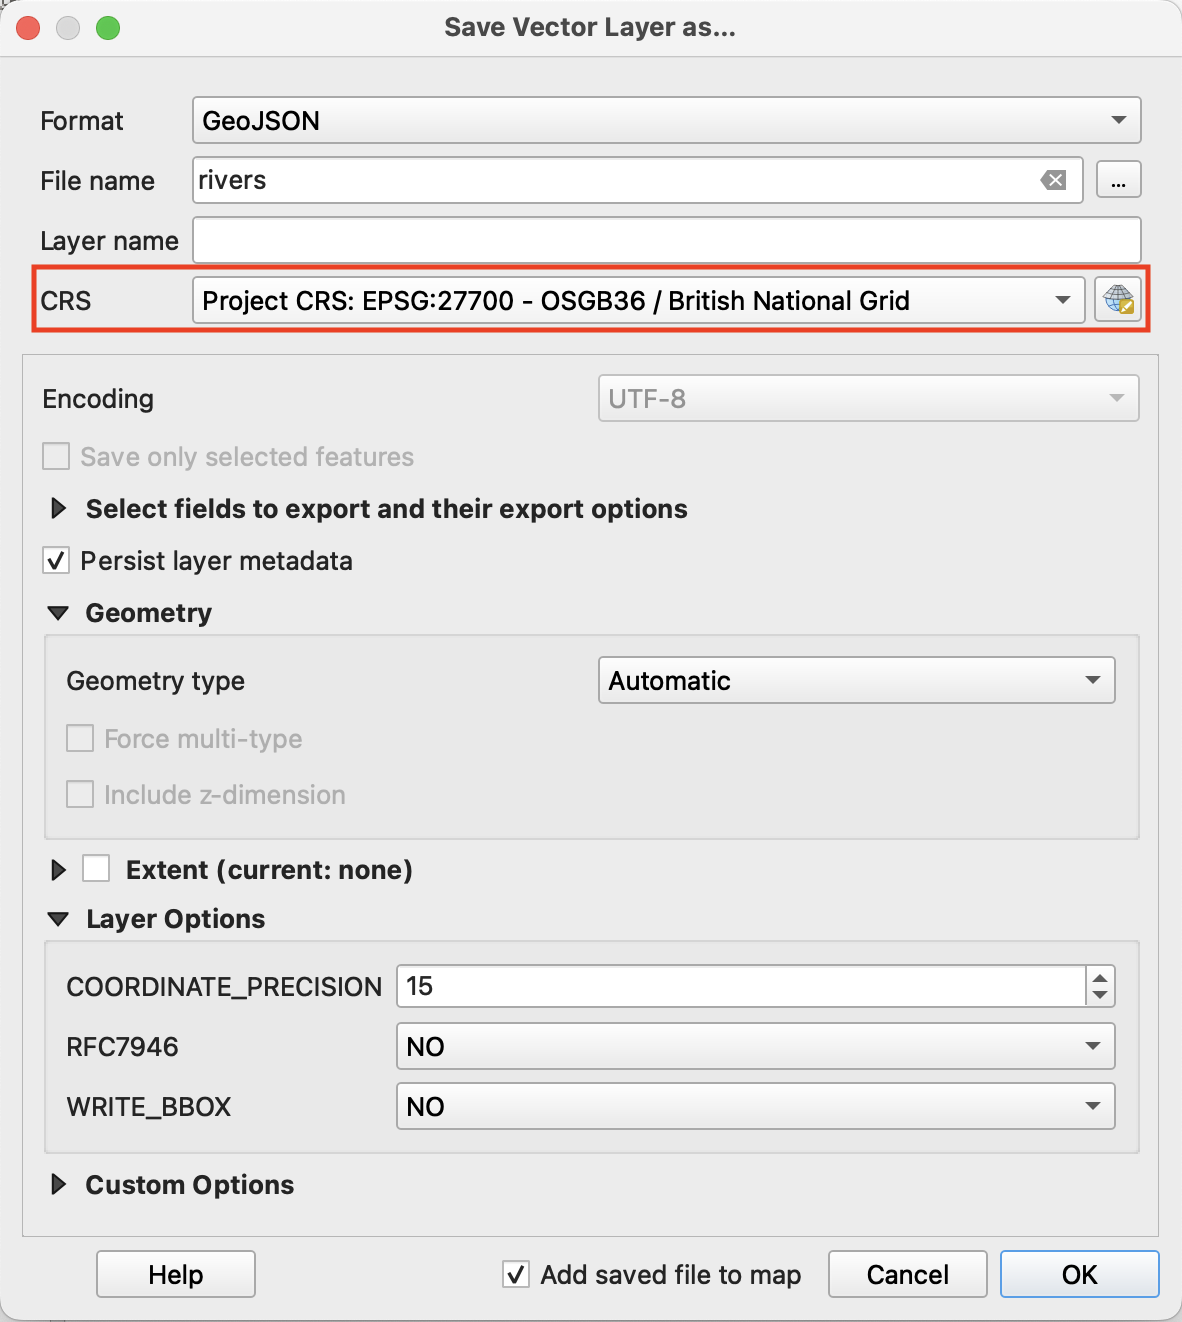
\includegraphics[width=\columnwidth]{figure/qgis/export_rivers.png}
        \caption{QGIS interface, exporting all rivers using the OSGB36 CRS in GeoJSON.}
        \label{fig:export_rivers}
    \end{figure}

    \begin{figure}[tbh!]
        \centering
        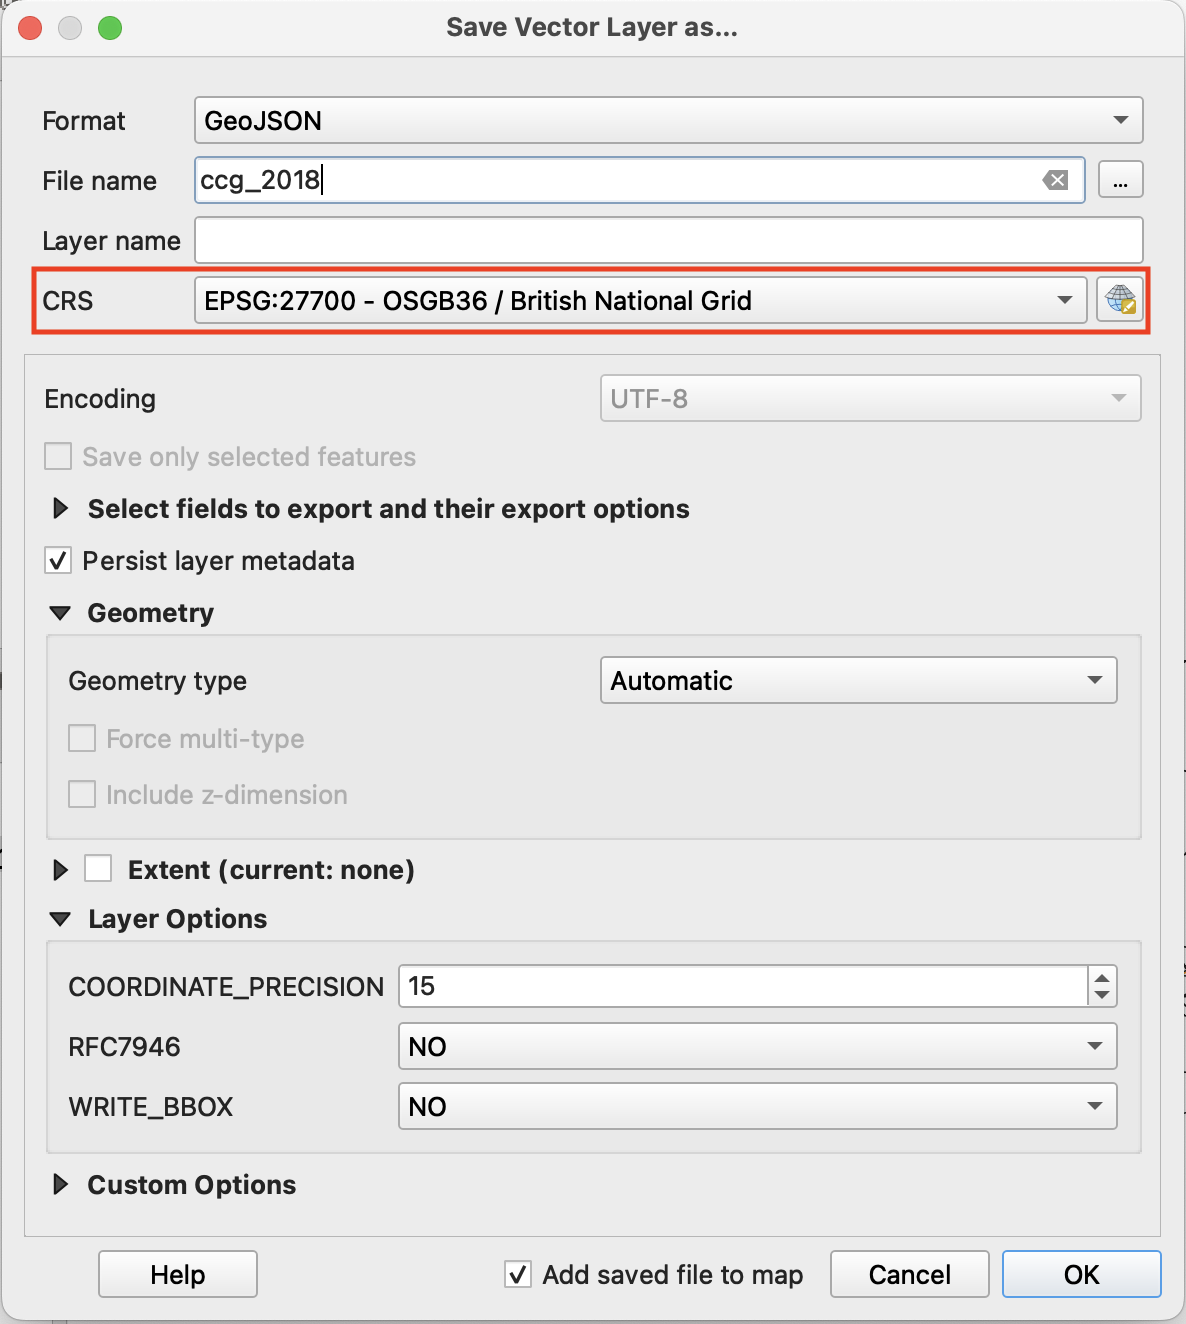
\includegraphics[width=\columnwidth]{figure/qgis/export_ccgs.png}
        \caption{QGIS interface, exporting all NHS CCGs using the OSGB36 CRS in GeoJSON.}
        \label{fig:export_ccgs}
    \end{figure}

}

\subsection{Merge Shapefiles and Reduce File Size}

We then merge two layers into one layer, and export it in the TopoJSON format using Mapshaper \cite{blochMapshaper}. Mapshaper also supports the simplification of GeoJSON shapefiles. See \autoref{fig:export_topojson}.

{
    \begin{figure}[tbh!]
        \centering
        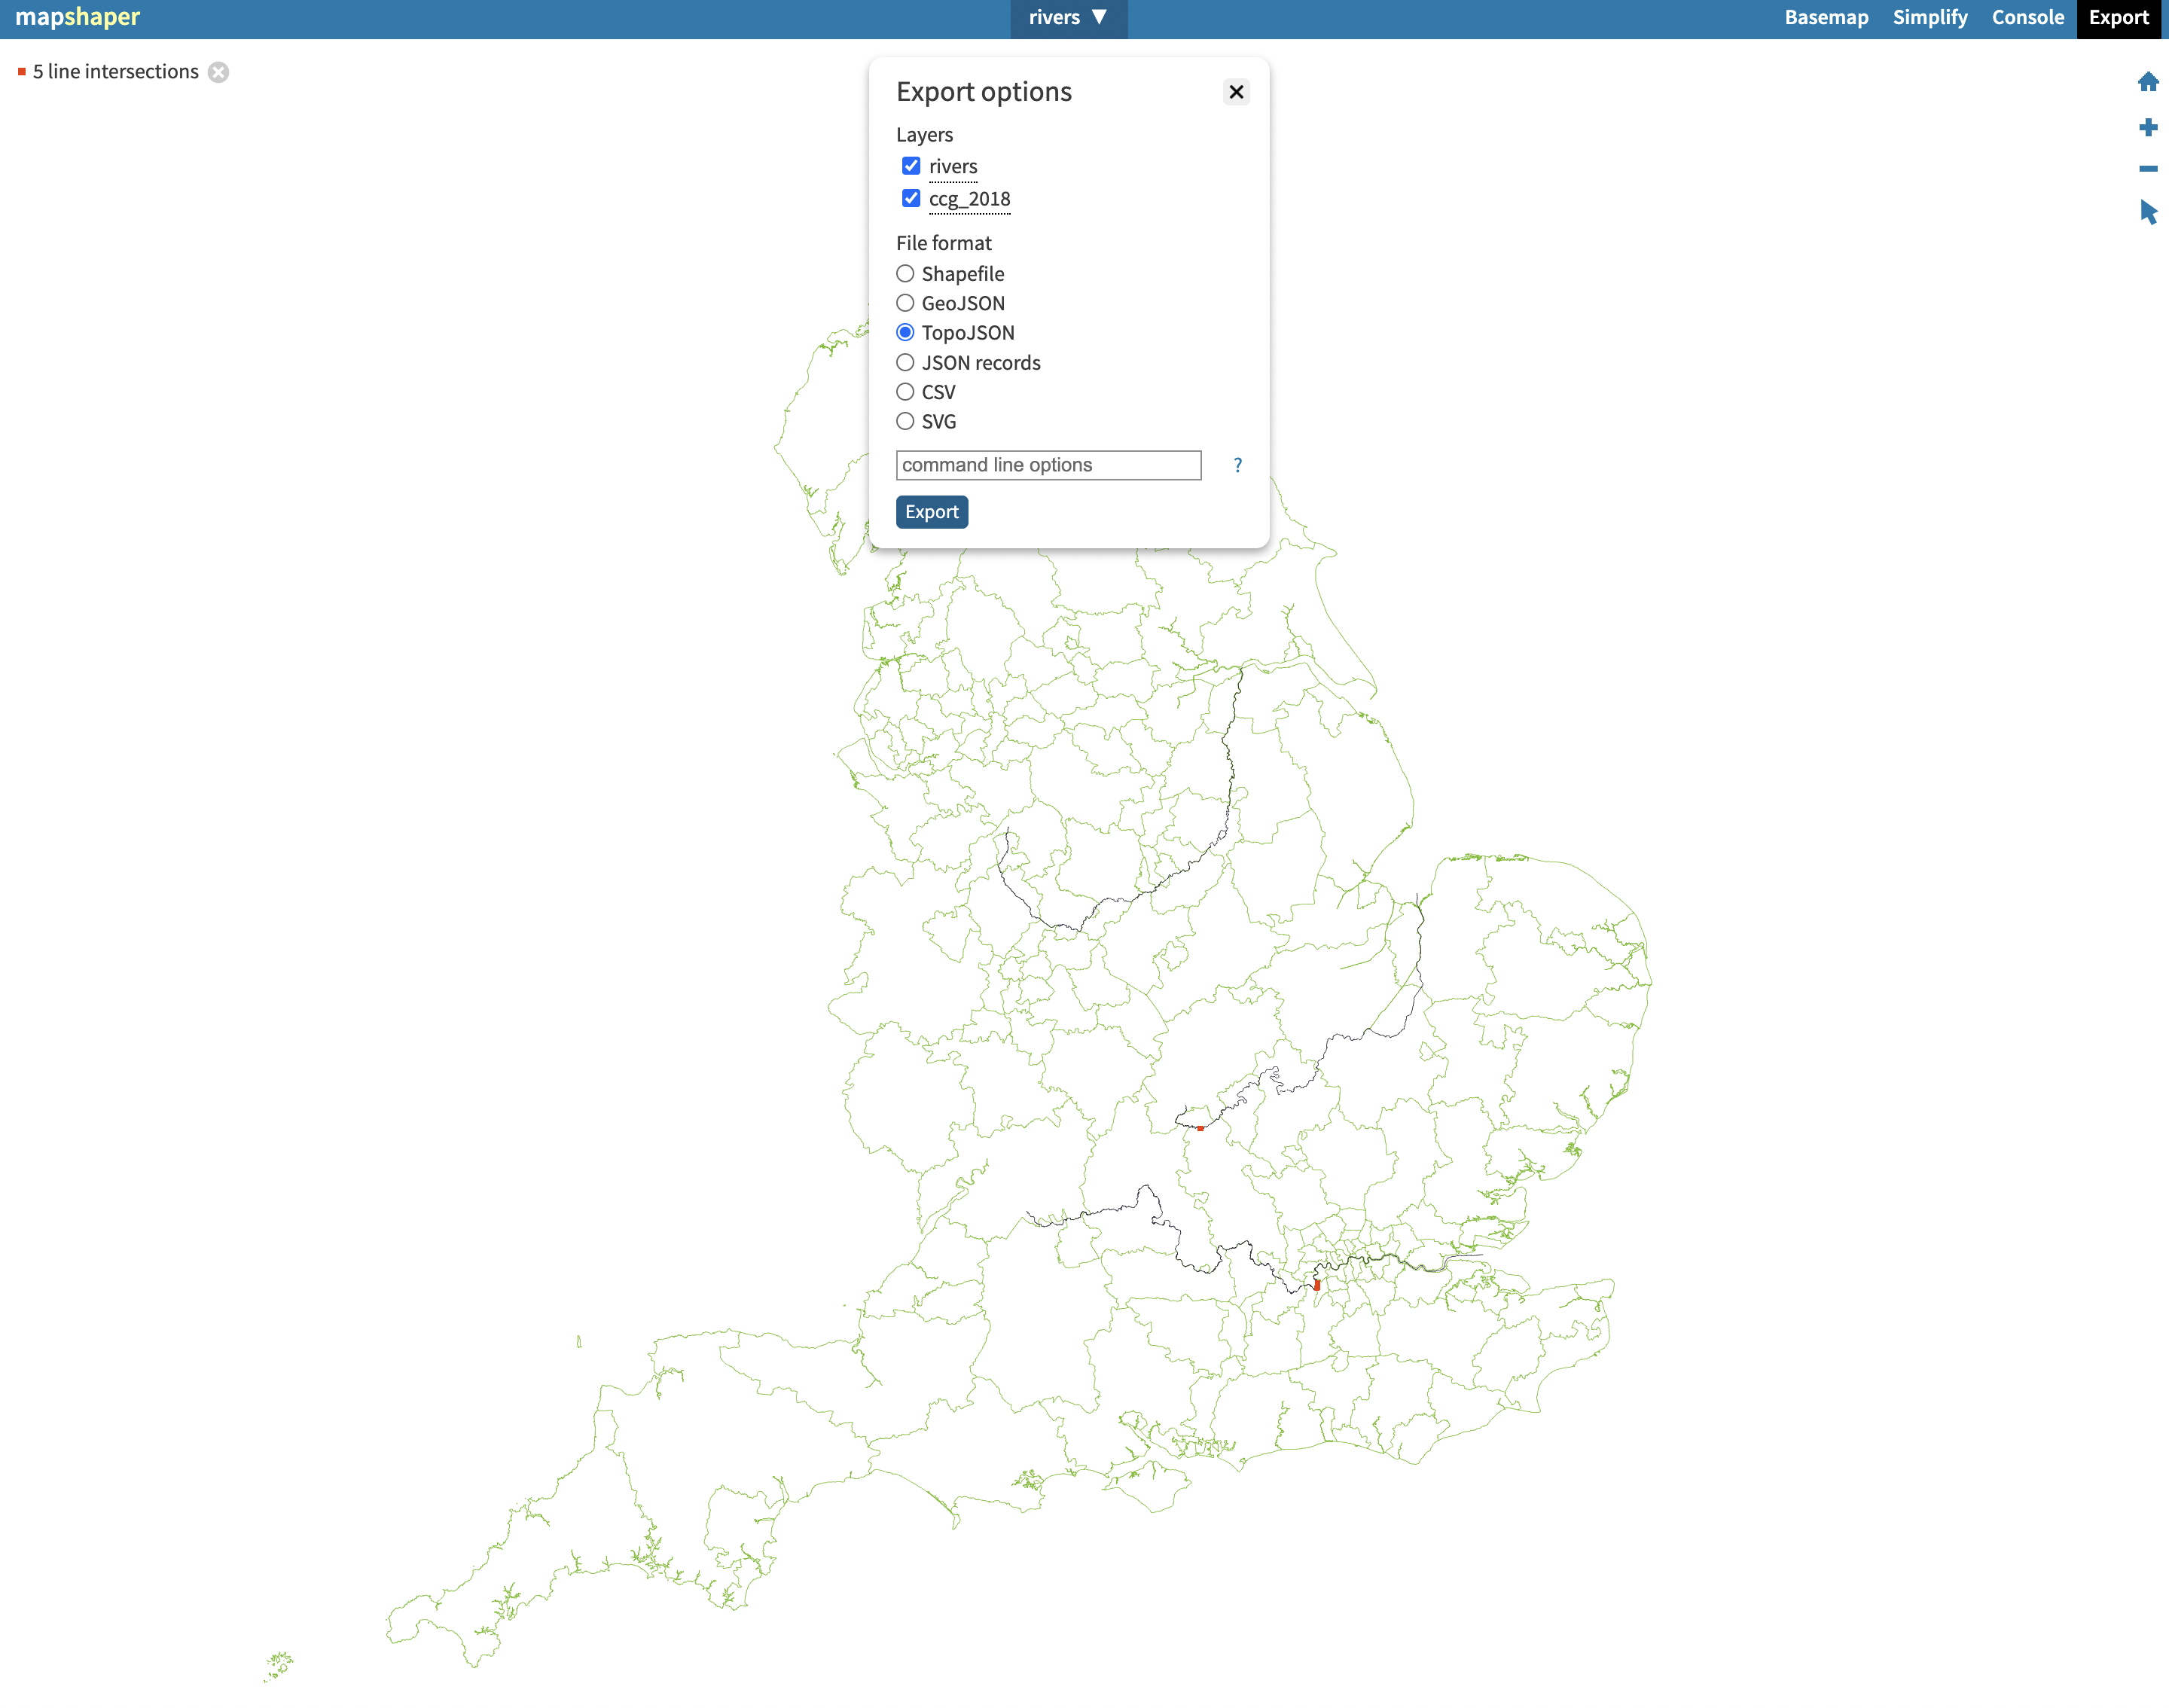
\includegraphics[width=\columnwidth]{figure/qgis/export_topojson.png}
        \caption{Mapshaper interface, merging all rivers with NHS CCGs into one layer, and export the merged layer in TopoJSON.}
        \label{fig:export_topojson}
    \end{figure}
}

\subsection{Pre-processing Result}

\autoref{table:pre-processing_result} shows the pre-processing result. The reduction in file size is significant and greatly reduces the initialization time of our implementation.

{
\renewcommand{\arraystretch}{1.5}
\begin{table}[!tb]
	\centering
	\resizebox{\columnwidth}{!}{
		\begin{tabulary}{\columnwidth}{|*{4}{l|}}
			\hhline{~|*{3}{-}}
			\multicolumn{1}{c|}{\textbf{Shapefile}} &
			\cellcolor{Mycolor2}\textbf{Original} &
			\cellcolor{Mycolor2}\textbf{GeoJSON} &
			\cellcolor{Mycolor2}\textbf{TopoJSON} \\
			\hline
			Rivers & 2.0 MB (GeoJSON) & 1.4 MB & -  \\
			\hline
			NHS CCGs & 46.6 MB (.shp, Esri vector shapefile) & 140.2 MB & -  \\
			\hline
			Merged & - & - & 16.3 MB \\
			\hline
		\end{tabulary}
	}
	\caption{The file size is reduced by 88.5\% from the original size.}
	\label{table:pre-processing_result}
\end{table}
}

\clearpage

\section{Procedure: DerivePoint}

% \begin{noindent}

    \begin{algorithm}[tbh!]
        \caption{Procedure to derive a point based an edge and a distance.}\label{alg:derive corridor point}
        \textbf{Input:} \\
        $ \Edge \gets $ the edge used to derive the new point \\
        $ \Distance \gets $ the distance between $ \PointP $ and $ \EdgeStart $ \\

        \textbf{Output:} \\
        A point, $ \PointP $, that is distance $ \Distance $ away from $ \EdgeStart $. \\
    
        \textbf{Local variables:} \\
        $ \dx, \dy \gets $ the differences in $ x, y $ for $ \EdgeStart $ and $ \EdgeEnd $ \\
    
        \begin{algorithmic}[1]
            \Procedure{DerivePoint}{$ \Edge $, $ \Distance $}
                \State $ \dx \gets \EdgeStart.x - \EdgeEnd.x $
    
                \State $ \dy \gets \EdgeStart.y - \EdgeEnd.y $
    
                \State $ \PointP.x \gets \frac{\dx}{\sqrt{\dx^2 + \dy^2}} \cdot \Distance $
    
                \State $ \PointP.y \gets \frac{\dy}{\sqrt{\dx^2 + \dy^2}} \cdot \Distance $
    
            \State \Return{$ \PointP $}
    
            \EndProcedure
    
        \end{algorithmic}
    \end{algorithm}
    
%\end{noindent}

\section{Procedure: DeriveParallelEdge}

% \begin{noindent}

\begin{algorithm}[tbh!]
    \caption{Procedure to derive an edge, $ \EdgeParallel $, that is parallel to $ \Edge $ with a distance of $ \Distance $.}\label{alg:derive corridor edge}

    \textbf{Input:} \\
    $ \Edge \gets $ the edge used to derive the parallel edge $ \EdgeParallel $ \\
    $ \Distance \gets $ the shortest distance between $ \Edge $ and $ \EdgeParallel $ \\

    \textbf{Output:} \\
    An edge, $ \EdgeParallel $, that is parallel to $ \Edge $ with a distance of $ \Distance $. \\

    \textbf{Local variables:} \\
    $ \dx, \dy \gets $ the differences in $ x, y $ for $ \EdgeStart $ and $ \EdgeEnd $ \\
    $ \Scale \gets $ the scale of $ \frac{\Distance}{\sqrt{\dx^2 + \dy^2}} $ \\

    \begin{algorithmic}[1]
        \Procedure{DeriveParallelEdge}{$ \Edge $, $ \Distance $}
            \State $ \dx \gets \EdgeStart.x - \EdgeEnd.x $

            \State $ \dy \gets \EdgeStart.y - \EdgeEnd.y $

            \State $ \Scale \gets \frac{\Distance}{\sqrt{\dx^2 + \dy^2}} $

            \State $ \EdgeParallel.start.x \gets \Scale \cdot -\dy + \EdgeStart.x $

            \State $ \EdgeParallel.start.y \gets \Scale \cdot \dx + \EdgeStart.y $

            \State $ \EdgeParallel.end.x \gets \Scale \cdot -\dy + \EdgeEnd.x $

            \State $ \EdgeParallel.end.y \gets \Scale \cdot \dx + \EdgeEnd.y $

        \State \Return{$ \EdgeParallel $}

        \EndProcedure

    \end{algorithmic}
\end{algorithm}

%\end{noindent}

\end{document}
